\documentclass[10pt]{beamer}

\mode<presentation>
{
  \usetheme[height=1.25cm]{Madrid}
  \setbeamertemplate{navigation symbols}{}
  \setbeamercolor{alerted text}{fg=illini}
}
\usebackgroundtemplate{
\includegraphics[width=\paperwidth,height=\paperheight]{uc-background}}

\usepackage[english]{babel}
\usepackage{epsfig,subfigure,bm}
\usepackage{multimedia}
\usepackage{psfrag}
\usepackage{animate}

%%%%%% Begin of my macros and options

\setbeamertemplate{section in toc shaded}[default][55]
\setbeamertemplate{subsection in toc shaded}[default][55]
\setbeamercolor{block title}{fg=white,bg=illini}
\setbeamercolor{block body}{fg=black,bg=mygrey}

\setbeamercolor{emphprimary}{fg=CBlue}
\setbeamercolor{emphsecondary}{fg=illini}
\setbeamercolor{emphtertiary}{fg=mygreen}
\definecolor{darkForestGreen}{rgb}{.1,1,.1}
\definecolor{veryLightGray}{rgb}{.9,.9,.9}
\definecolor{greenApple}{rgb}{.3,.9,.3}

\setbeamercolor{frametitle}{bg=CBlue}   
\setbeamercolor{title}{bg=CBlue}

\usepackage{amsmath,amssymb,amsxtra,amsthm}
\usepackage{algorithm,algorithmic}
\usepackage{natbib}
\usepackage{bibentry}
\usepackage{xspace}
\usepackage{changepage}

\pdfmapfile{+sansmathaccent.map}

\definecolor{myblue}{rgb}{.2,.2,.7}
\definecolor{myred}{rgb}{.7,.2,.2}
\definecolor{mygreen}{rgb}{.2,.7,.2}
\definecolor{mygrey}{rgb}{0.9,0.9,0.9}
\definecolor{CBlue}{cmyk}{1,0.25,0,0}
\definecolor{illini}{rgb}{0.98,0.4,0.05}
\definecolor{black}{cmyk}{0,0,0,1}

\newcommand{\myemph}[1]{{\usebeamercolor[fg]{emphprimary}
    \textbf{#1}}}
\newcommand{\myemphalt}[1]{{\usebeamercolor[fg]{emphsecondary}
    \textbf{#1}}}

\graphicspath{{figs/}}

\title[Math for Robotics] % (optional, use only with long paper titles)
{CSE276C - Subspace Methods}

\author[H.~I. Christensen] % (optional, use only with lots of authors)
{Henrik I.~Christensen}
% - Give the names in the same order as the appear in the paper.  -
% Use the \inst{?} command only if the authors have different
% affiliation.

\AtBeginSection[]
{
   \begin{frame}
       \frametitle{Outline}
       \tableofcontents[currentsection]
   \end{frame}
}

\institute[UCSD] % (optional, but mostly needed)
{
  \begin{minipage}[c]{.2\textwidth}
    
\includegraphics[width=.65\linewidth]{ucsealnew}%
  \end{minipage}%
  \begin{minipage}[c]{.6\textwidth}
    \small
%%    \begin{center}
      Computer Science and Engineering\\
      University of California, San Diego\\
      \myemph{\url{http://cri.ucsd.edu}}\\
%%    \end{center}

  \end{minipage}
%%  \vspace*{1ex}
}
%% - Use the \inst command only if there are several affiliations.
%% - Keep it simple, no one is interested in your street address.

\bigskip

\date[Oct 2024]% (optional, should be abbreviation of conference name)
{\small%
  October 2024}

\begin{document}

\nobibliography{/Users/hic/Dropbox/bibliography/bib-file}
\bibliographystyle{plain}

\begin{frame}[plain]
  \titlepage
\end{frame}

\begin{frame}
  \frametitle{Literature}
  \begin{itemize}
  \item Leonardis, A. and Bischof, H., 2000. ``Robust recognition
    using eigenimages''. {\bf Computer Vision and Image
      Understanding}, 78(1), pp.99-118.
  \item Largely adopted from ECCV tutorial by Leonardis and Bischof
  \end{itemize}
\end{frame}

\section{Introduction}

\begin{frame}
  \frametitle{Recognition of objects in clutter}
  \centerline{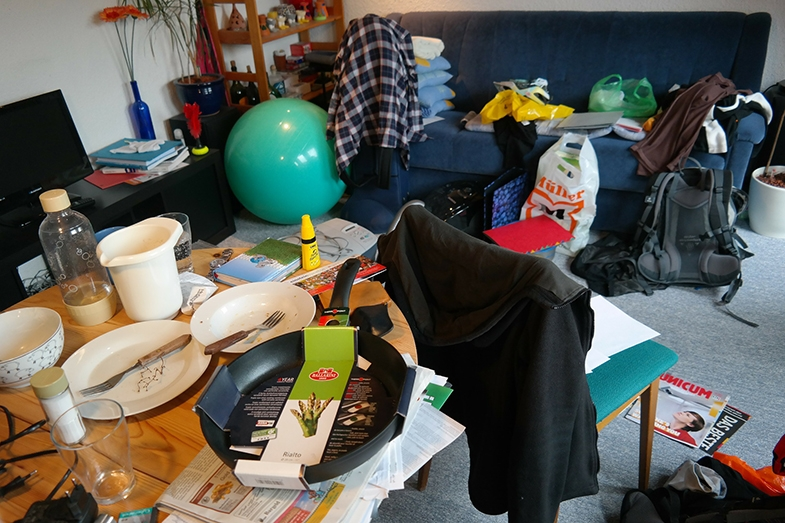
\includegraphics[width=9cm]{home-clutter}}
\end{frame}

\begin{frame}
  \frametitle{Recognition of objects in clutter}
  \centerline{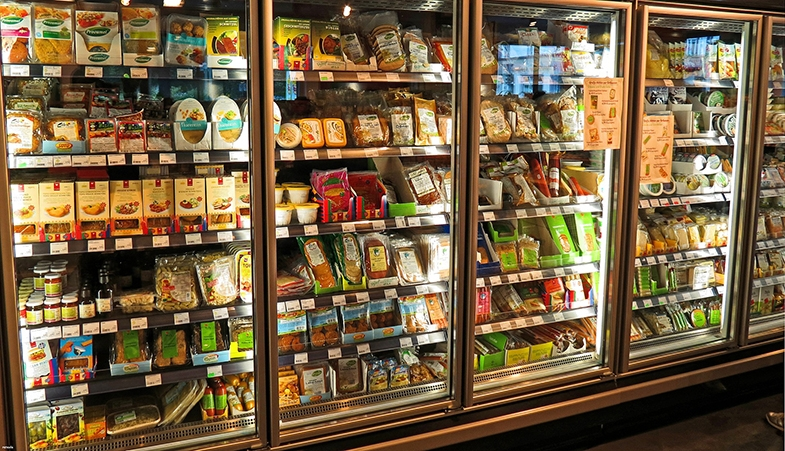
\includegraphics[width=9cm]{grocery-store}}
\end{frame}

\begin{frame}
  \frametitle{Typical tasks}
  \begin{itemize}
  \item Where can I find a can of coke? 
  \item Check the stove -- is it off? 
  \item Put away the groceries in the pantry? 
  \end{itemize}
\end{frame}

\section{Appearance based learning and recognition}
\label{sec:appearance}

\begin{frame}
  \frametitle{Object Representation}
  \begin{itemize}
  \item High-level Shape Models (e.g., Generalized Cylinders)
    \begin{itemize}
    \item Idealized images
    \item Texture Less
    \end{itemize}
  \item Mid-level Shape Models (e.g., CAD models, Superquadrics)
    \begin{itemize}
    \item More complex
    \item Well-defined geometry
    \end{itemize}
  \item {\color{red} Low-level Appearance Based Models} (e.g., Eigenspaces)
    \begin{itemize}
    \item Most complex
    \item Complicated shapes
    \end{itemize}
  \end{itemize}
\end{frame}

\begin{frame}
  \frametitle{A number of challenges}
  \center{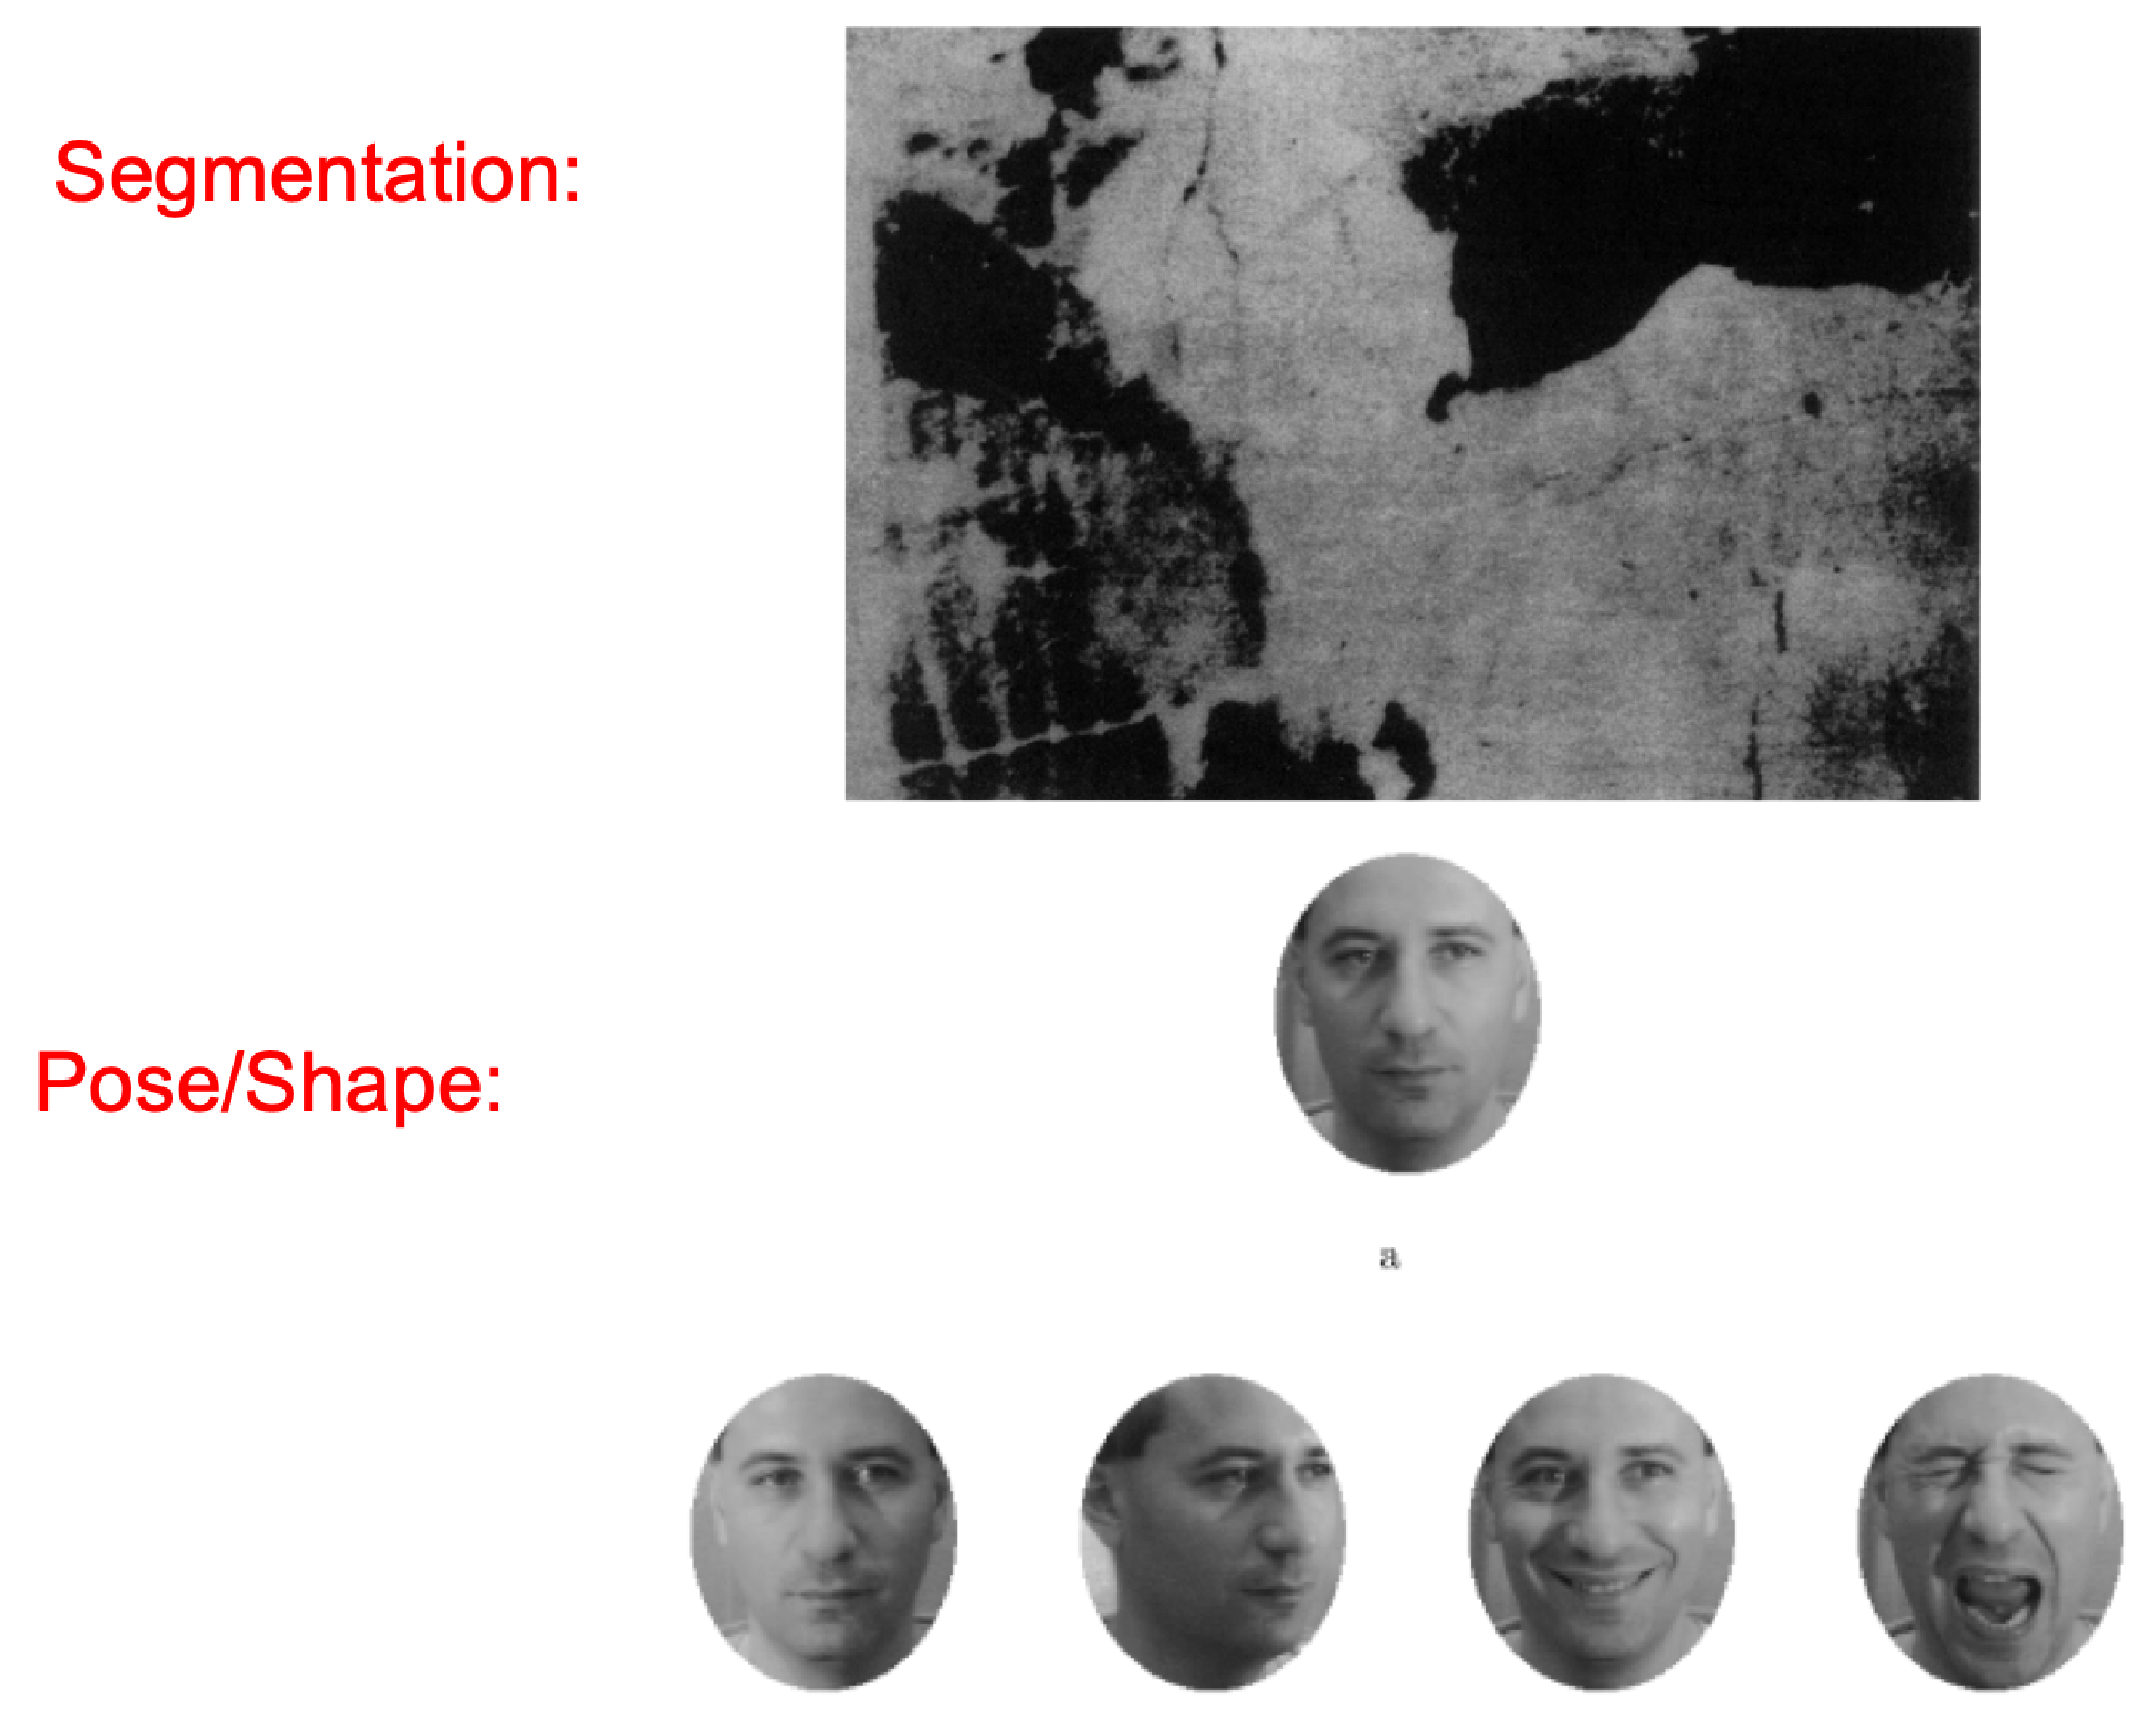
\includegraphics[height=6cm]{image-challenges}}
\end{frame}

\begin{frame}
  \frametitle{Changes in illumination}
  \center{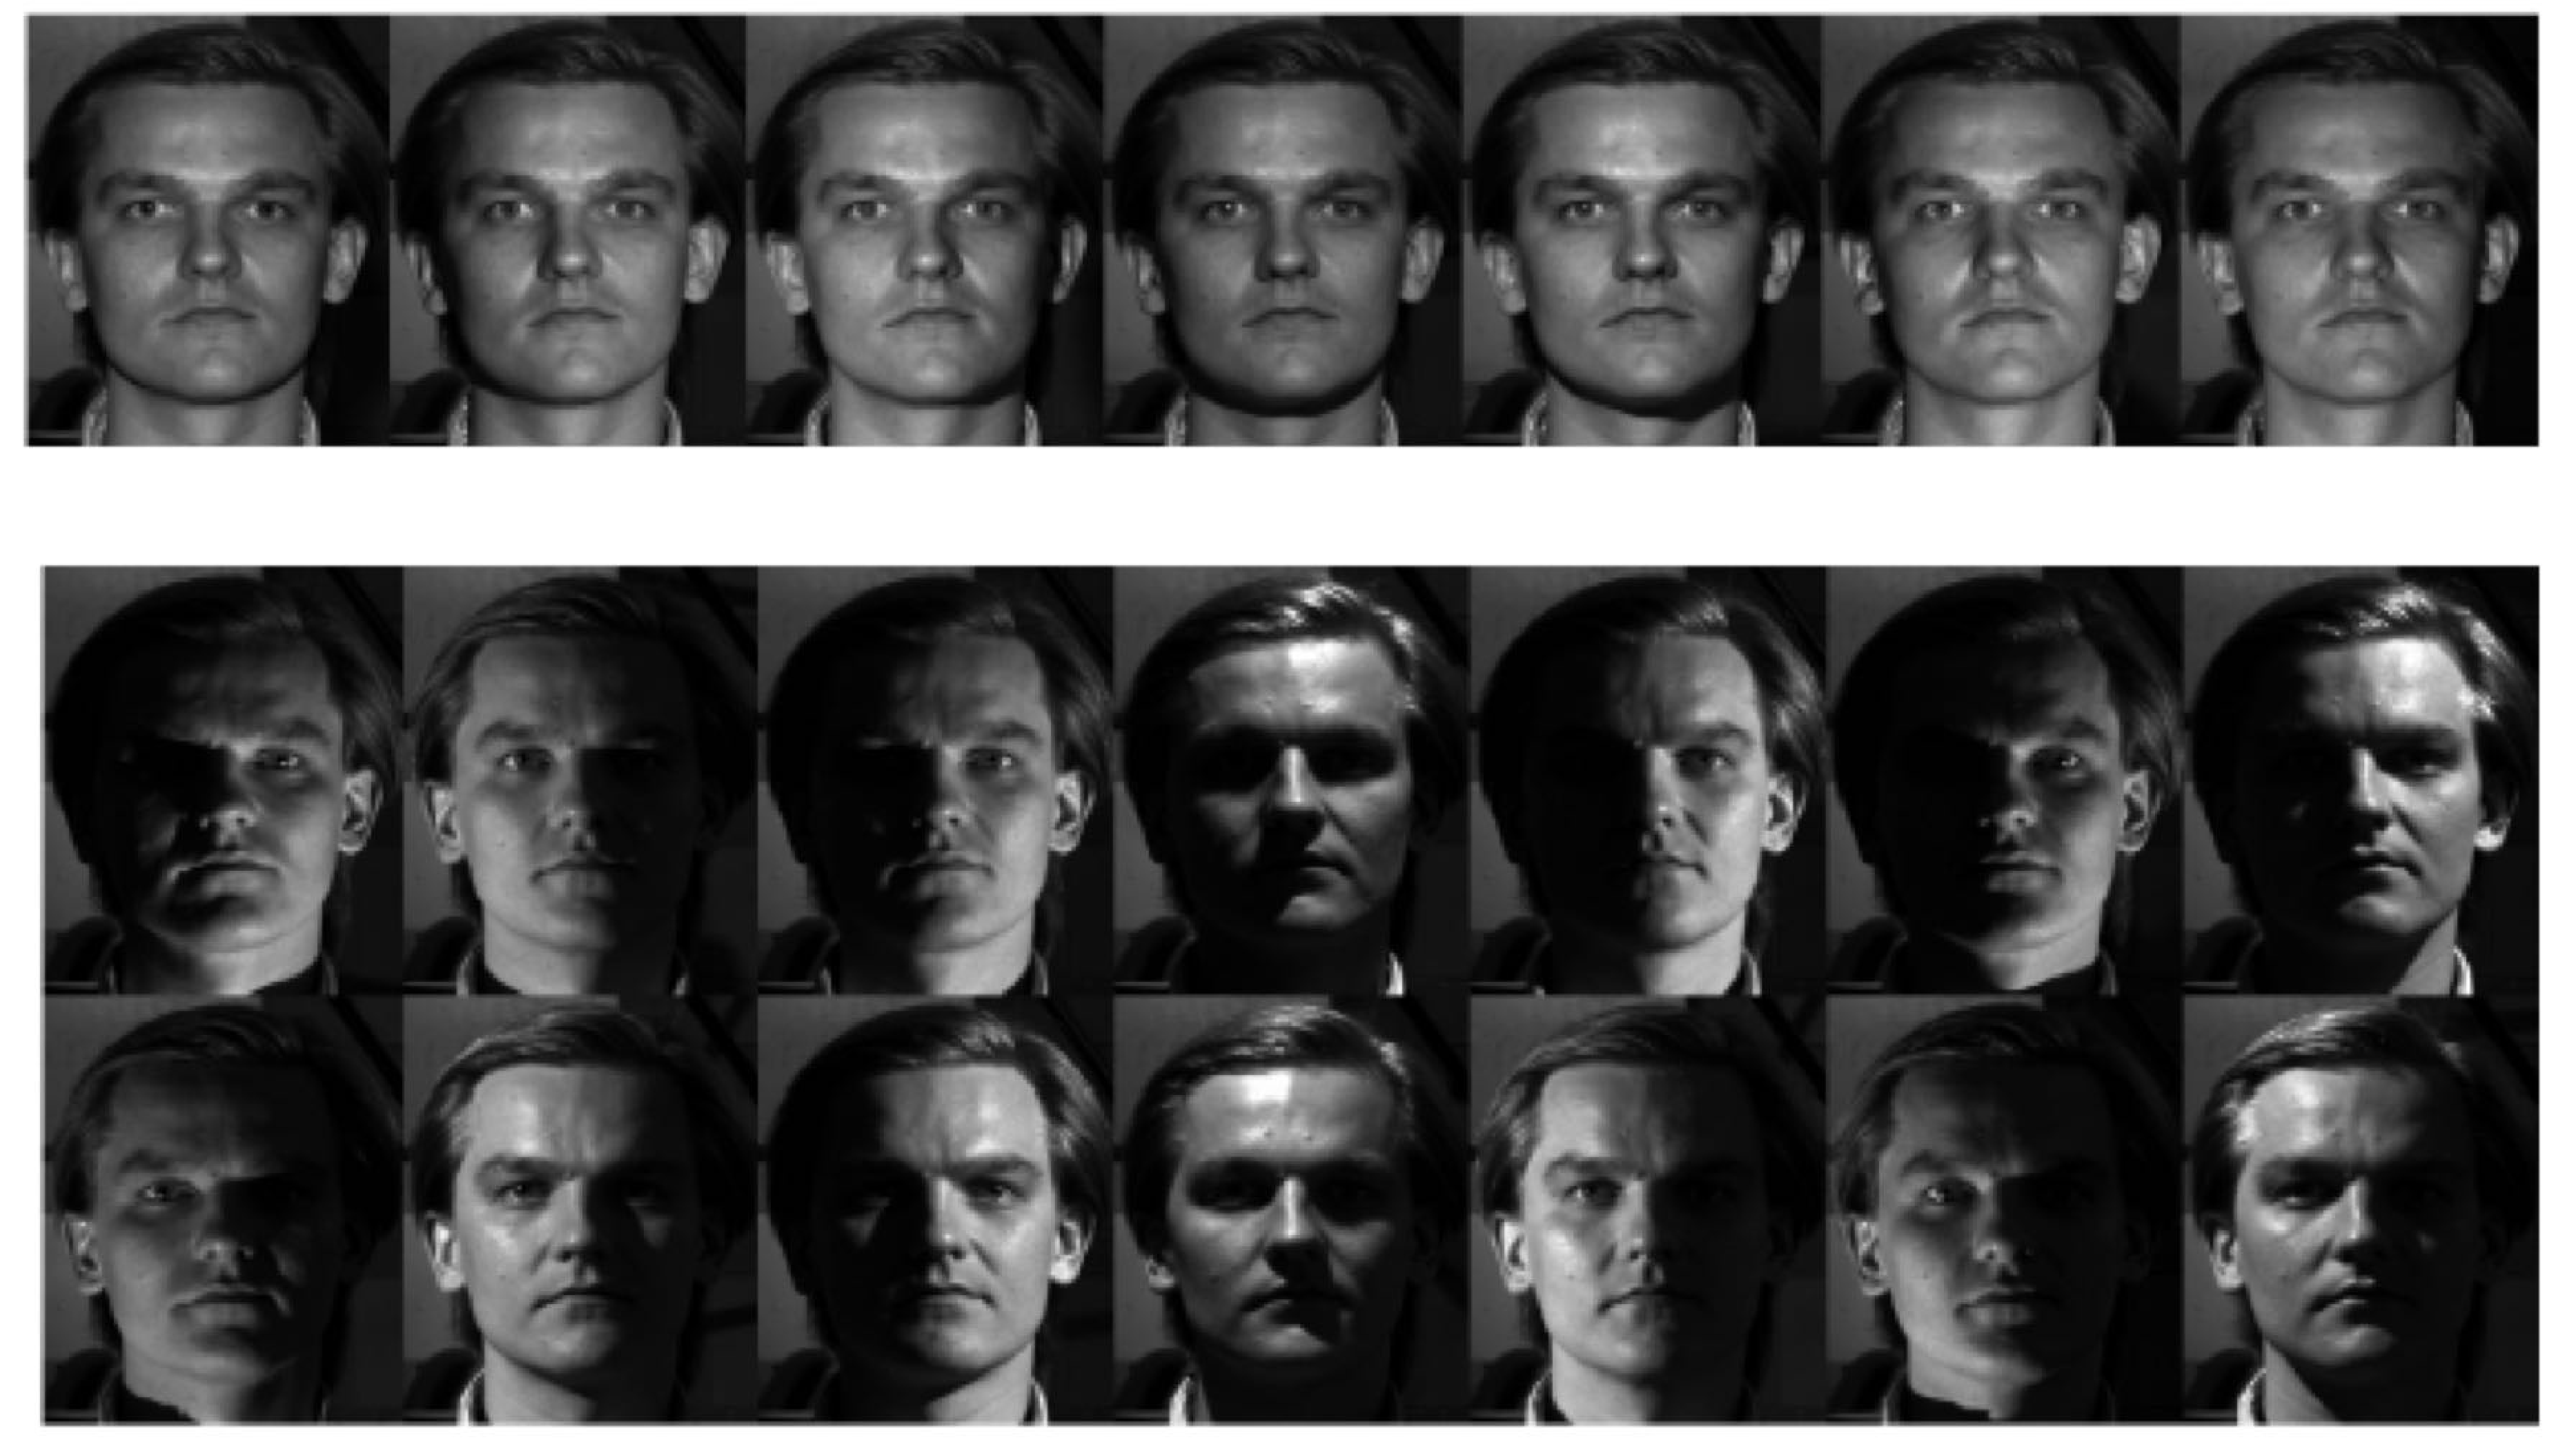
\includegraphics[height=6cm]{faces-illumination}}
\end{frame}

\begin{frame}
  \frametitle{The importance of context}
  \center{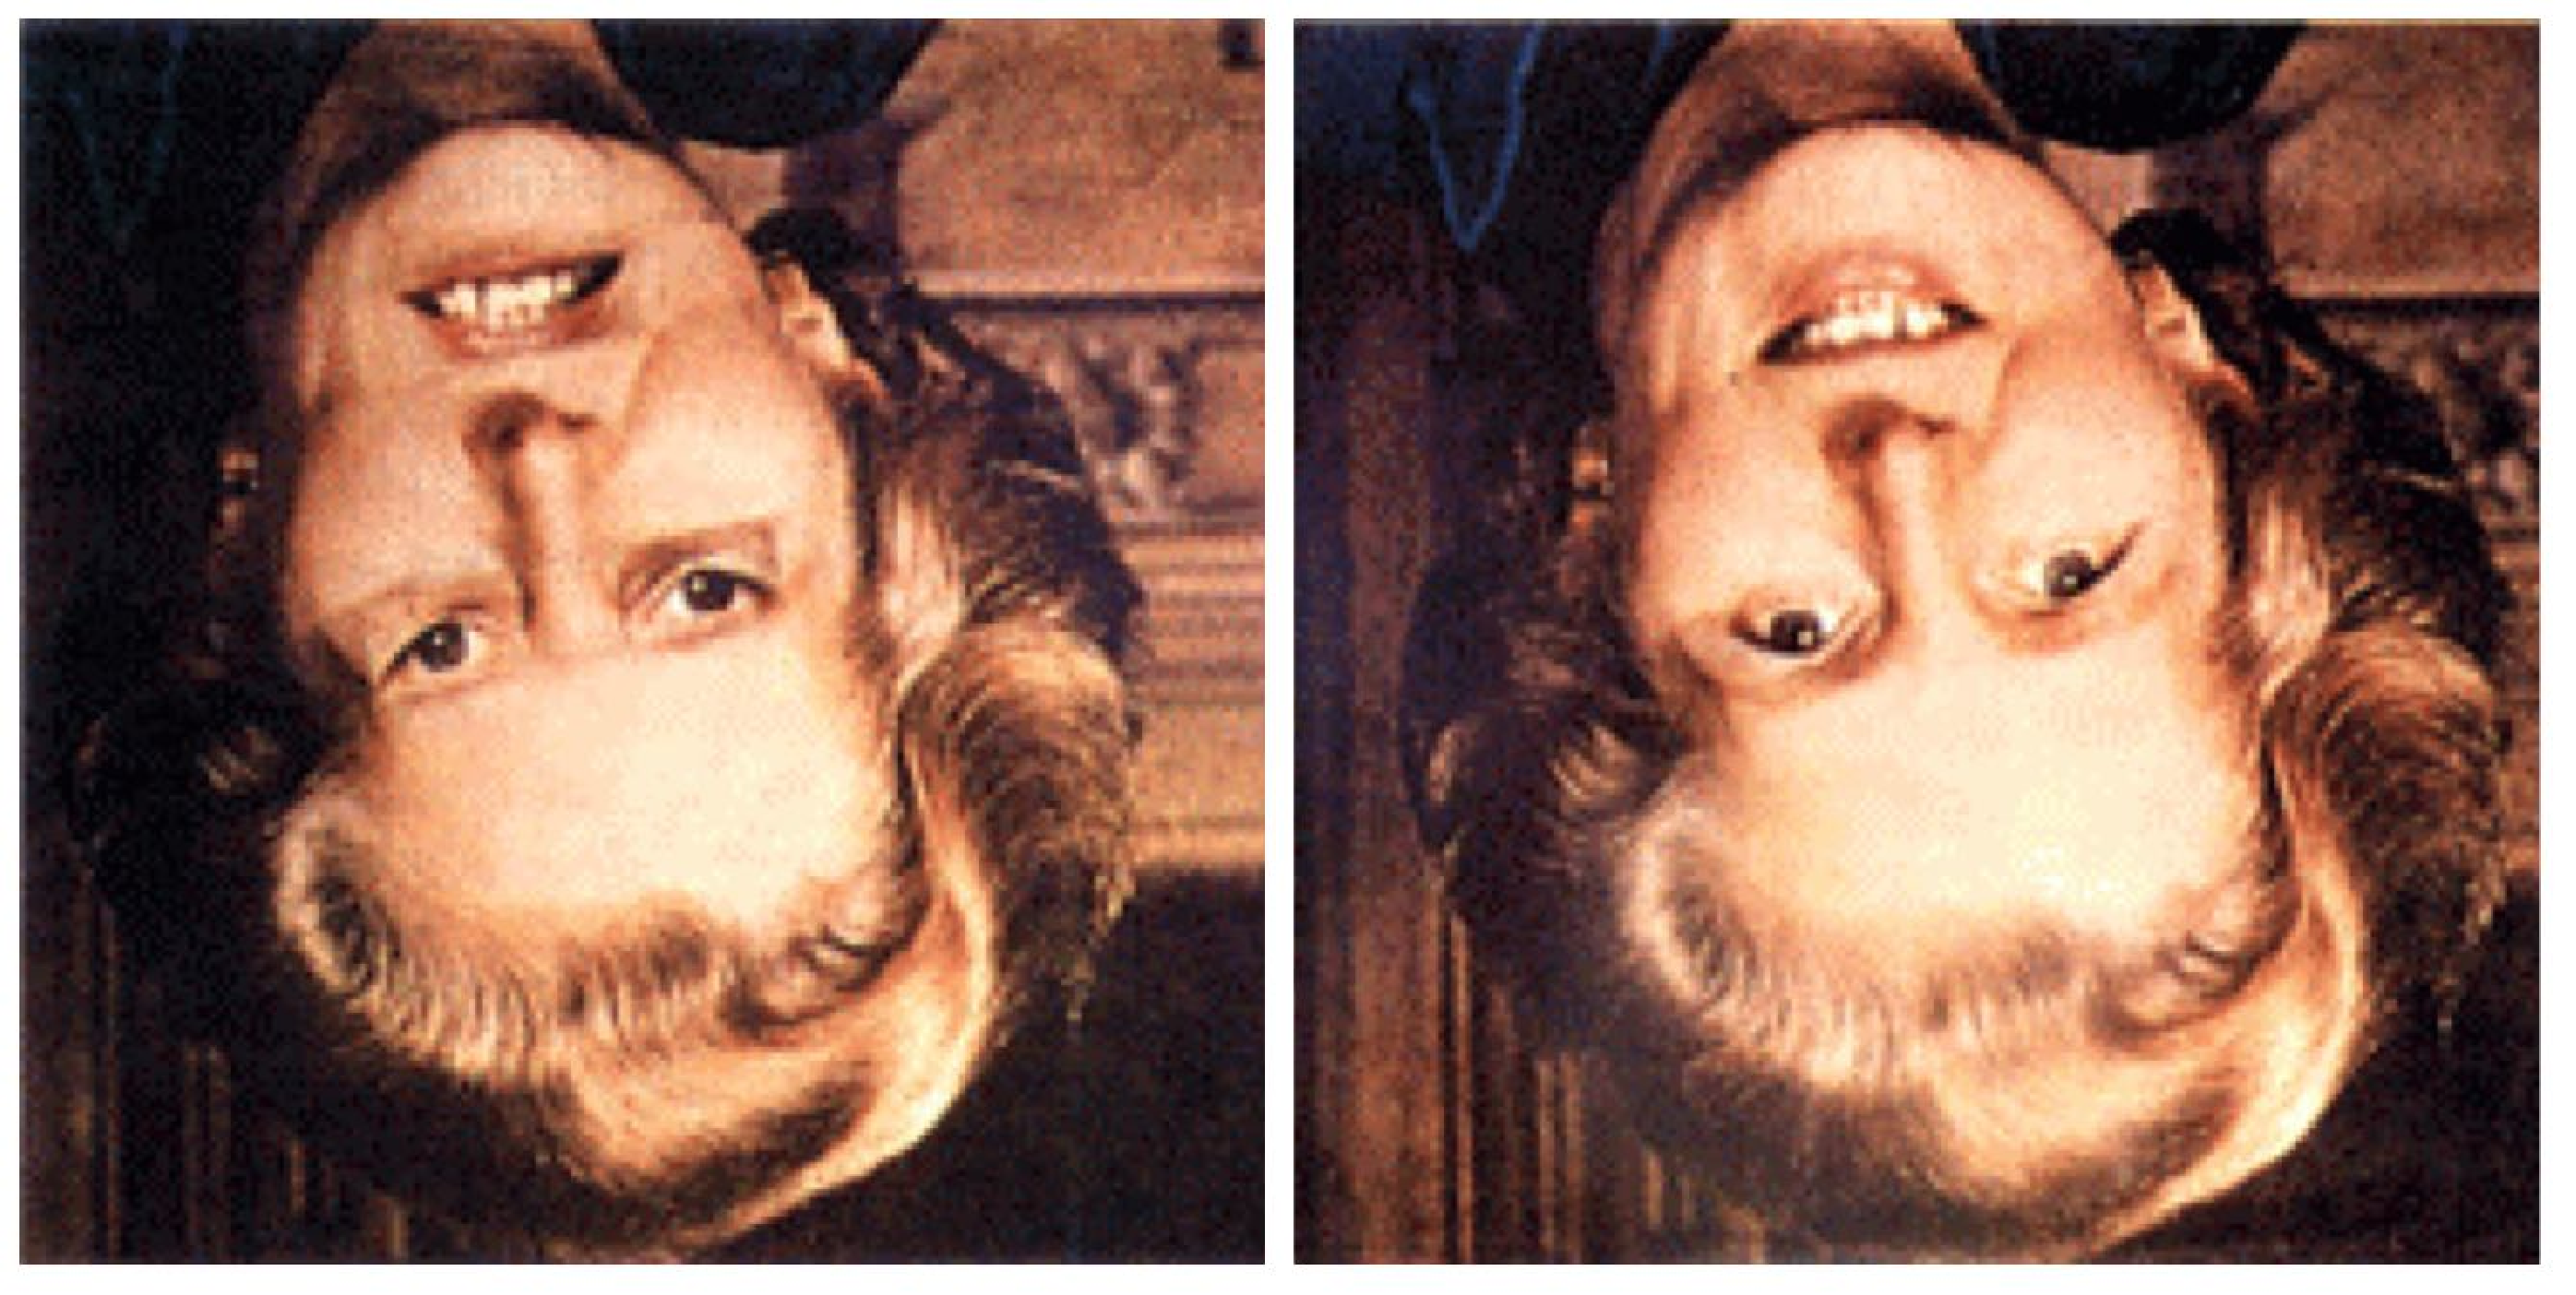
\includegraphics[height=6cm]{thatcher-up}}
\end{frame}

\begin{frame}
  \frametitle{The importance of context - see}
  \center{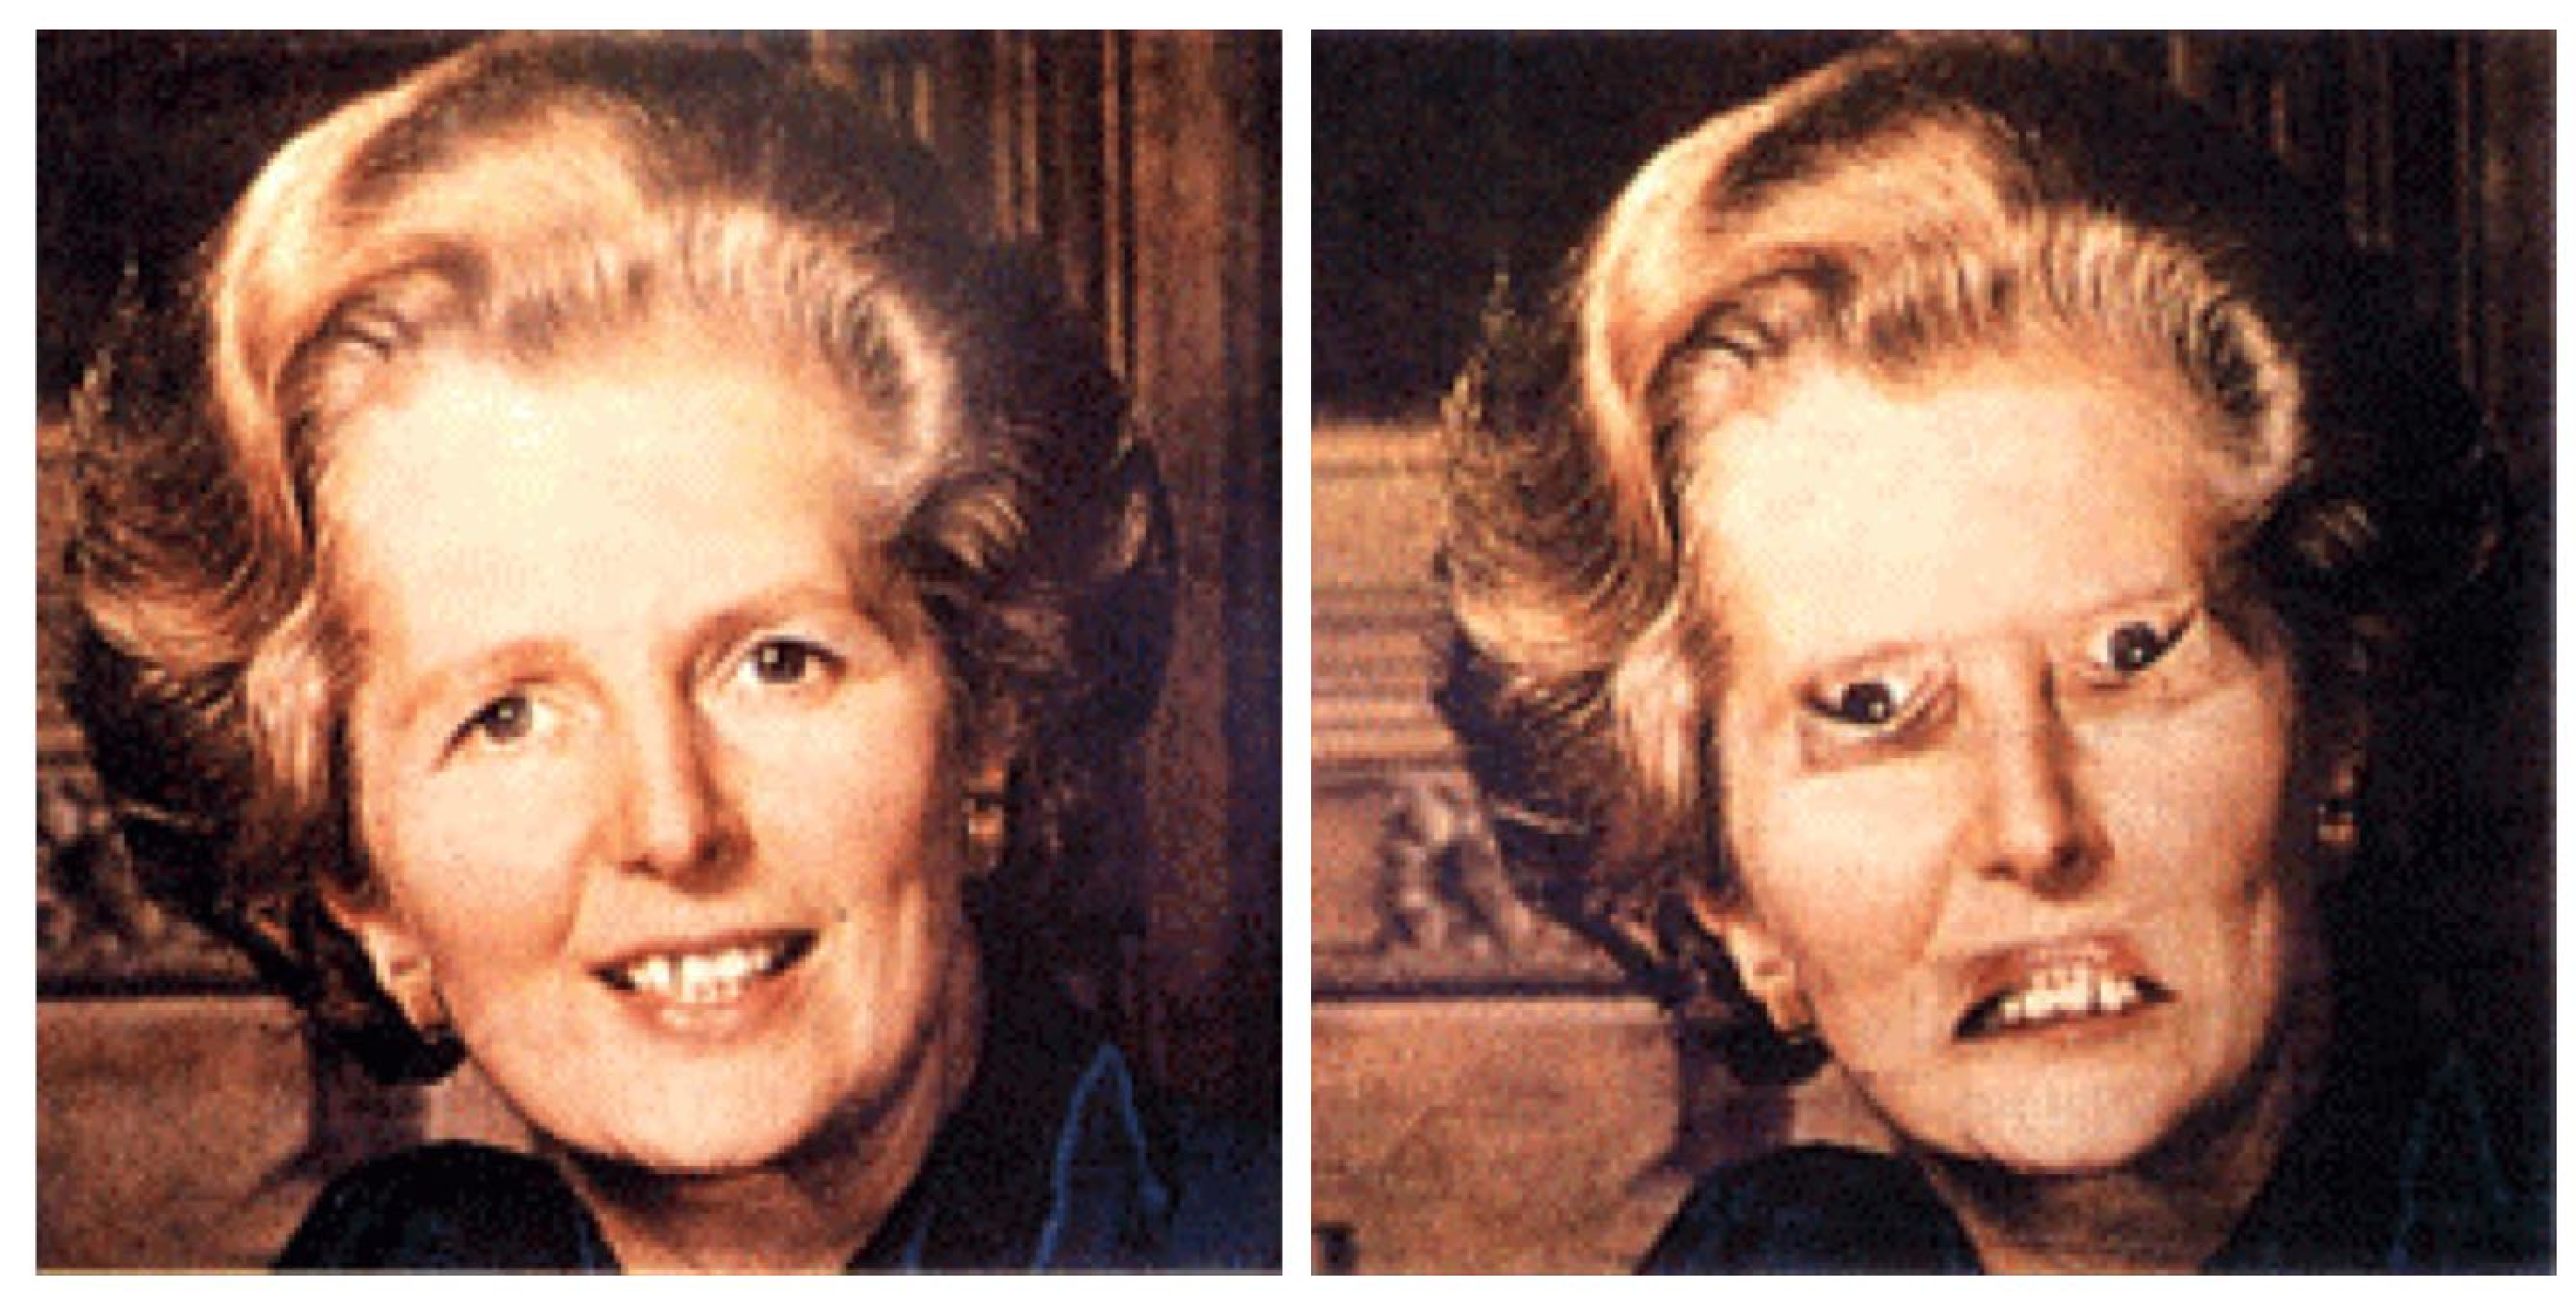
\includegraphics[height=6cm]{thatcher}}
\end{frame}

\begin{frame}
  \frametitle{Learning and recognition}
  \center{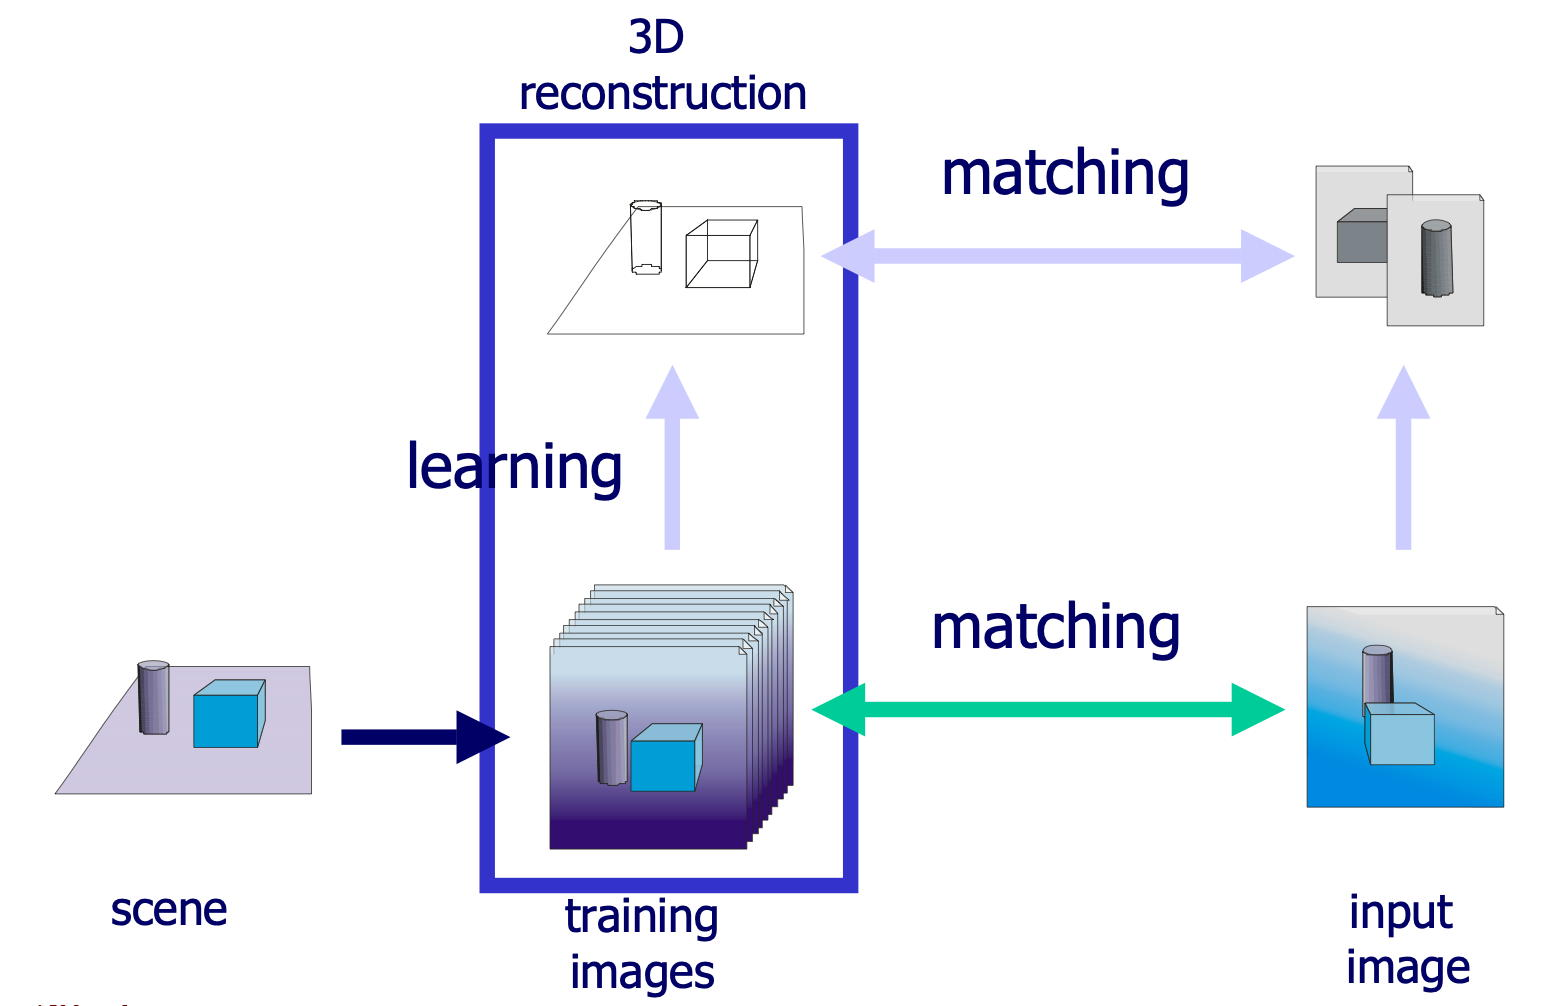
\includegraphics[height=6cm]{process-diagram}}
\end{frame}

\section{Appearance based method for visual object recognition}
\label{sec:appearance-rec}

\begin{frame}
  \frametitle{Appearance-based approaches}
  \begin{itemize}
  \item The abundance of image data gives a renewed interest in appearance-based approaches
  \item Combined effort of:
    \begin{itemize}
    \item Shape
    \item Reflectance properties
    \item Pose in the scene
    \item Illumination conditions / variations
    \end{itemize}
  \item Acquired through an automatic learning phase
  \item Well defined error characteristics
  \end{itemize}
\end{frame}

\begin{frame}
  \frametitle{Numerous use-cases}
  \begin{itemize}
  \item Face-recognition (eigen faces)
  \item Visual inspection
  \item Tracking and pose estimation for robotics
  \item Basic object tracking
  \item Planning of illumination
  \item Image spotting
  \item Mobile robot localization
  \item \ldots
  \end{itemize}
\end{frame}

\begin{frame}
  \frametitle{IDEA: Take a large number of image views}
  \centerline{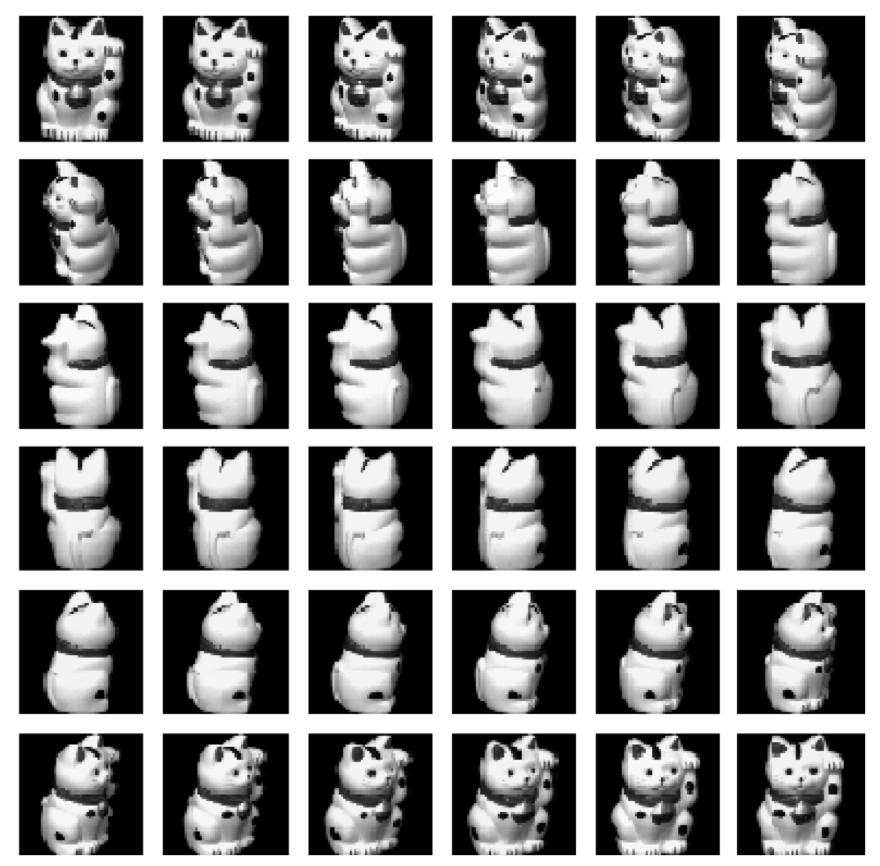
\includegraphics[height=6cm]{rotating-kitty}}
\end{frame}

\begin{frame}
  \frametitle{IDEA: Subspace Methods}
  \begin{itemize}
  \item Images are represented as points in an N-dimensional space
  \item Images only occupy a small fraction of the hyper-space
  \item Characterize the subspace / manifold spanned by the images
  \end{itemize}
  \centerline{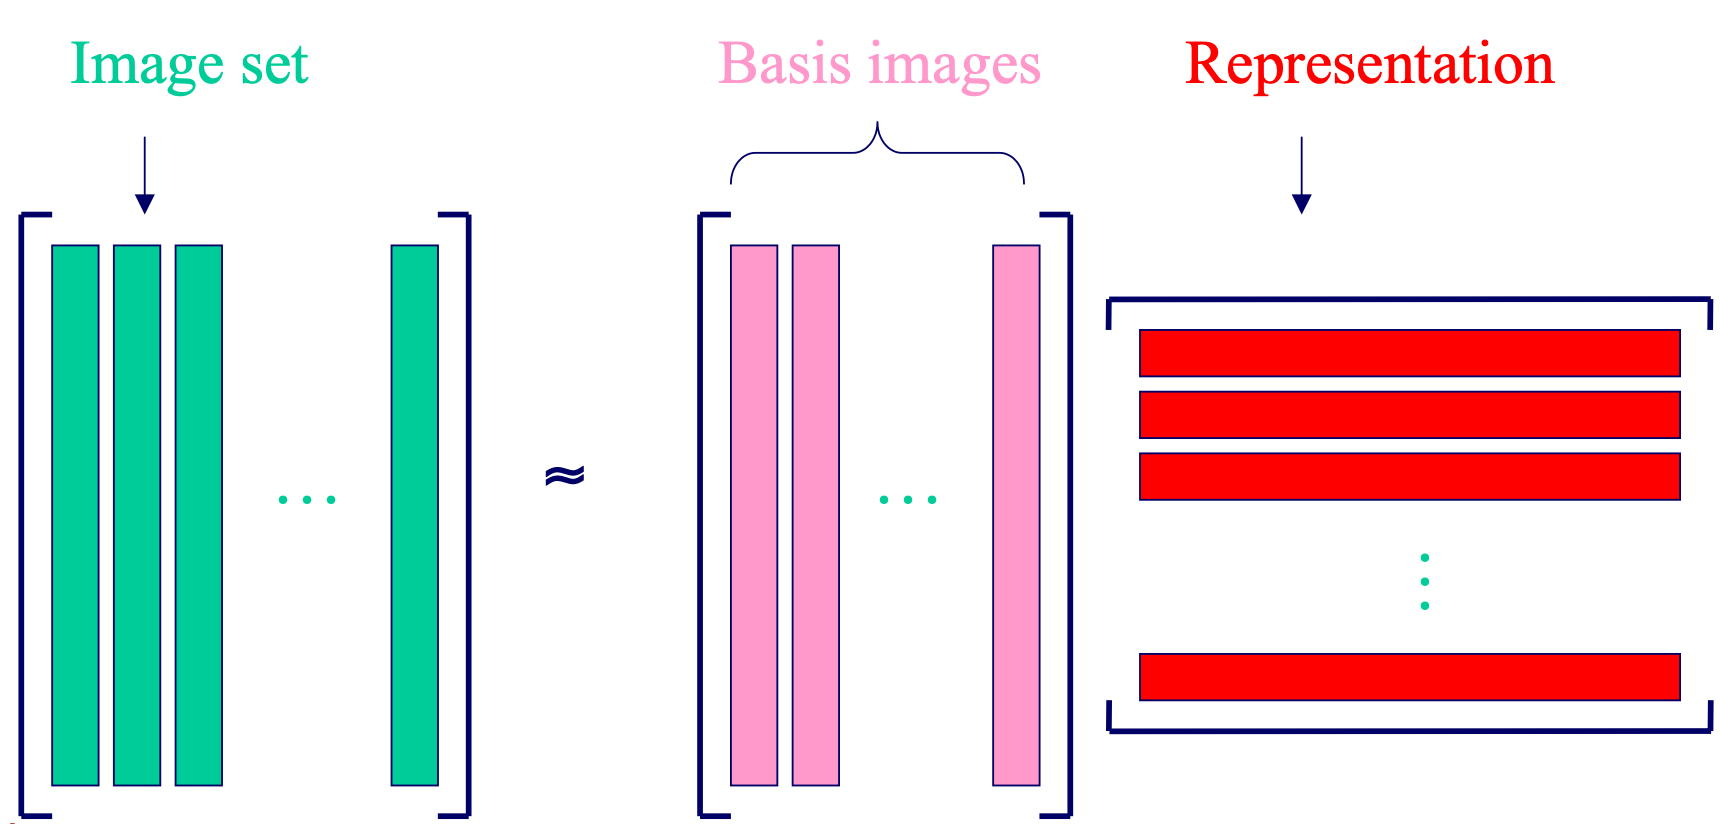
\includegraphics[height=4cm]{subspace-sketch}}
\end{frame}

\begin{frame}
  \frametitle{Multiple subspace methods}
  \begin{itemize}
  \item Optimal Reconstruction $\Rightarrow$ PCA
  \item Optimal Separation $\Rightarrow$ LDA
  \item Optimal Correlation $\Rightarrow$ CCA
  \item Independent Factors $\Rightarrow$ ICA
  \item Non-negative factorization $\Rightarrow$ NMF
  \end{itemize}
\end{frame}

\begin{frame}
  \frametitle{Image matching}
  \centerline{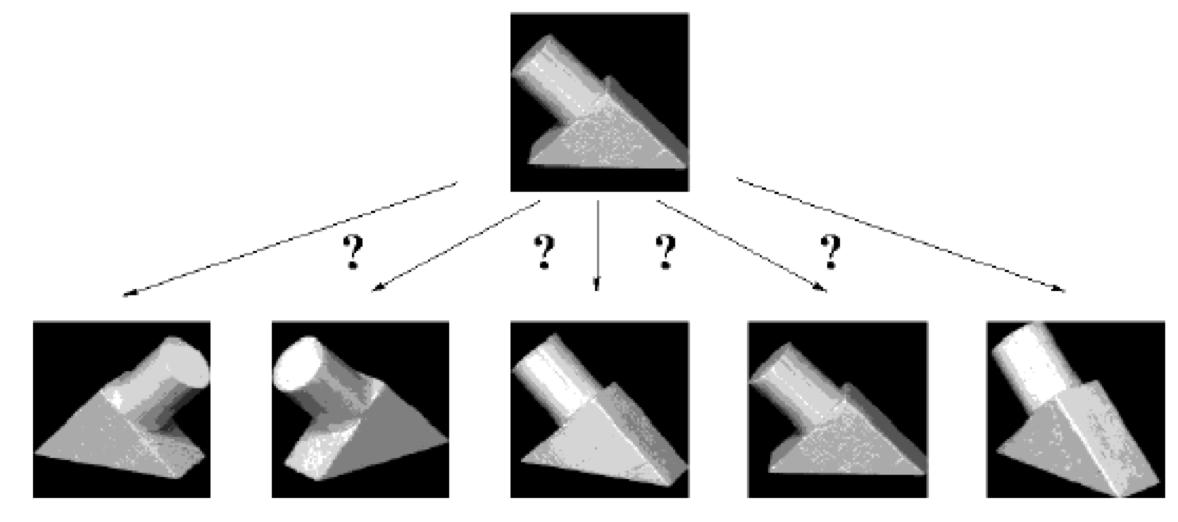
\includegraphics[height=4cm]{image-matching}}
  \[
    \rho = \frac{x^T y}{||x|| ||y||} \geq \Theta
  \]
  Or Normalized Images
  \[
    || x - y ||^2 \leq \Phi
  \]
\end{frame}

\begin{frame}
  \frametitle{Eigenspace representation}
  \begin{itemize}
  \item Image set (normalized, zero mean)
    \[ X = [ x_0 ~ x_1 ~ \ldots ~  x_{n-1} ] ; ~ X \in R^{m \times n} \]
  \item Looking for ortho-normal basis
    \[ U = [ u_0 ~ u_1 ~ \ldots ~ u_k ~ ] ; k \ll n \]
  \item Individual images are then a linear combination of basis vectors
    \[ x_i \approx \tilde{x}_i = \sum_{j=0}^k q_j(x_i) u_j \]
    \[ || x - y ||^2 \approx || \sum_{j=0}^k q_j(x) u_j -  \sum_{j=0}^k q_j(y) u_j ||^2 \]
    \[  || \sum_j q_j(x) - q_j(y) ||^2 \] 
  \end{itemize}
\end{frame}

\begin{frame}
  \frametitle{Choosing a basis function?}
  \begin{itemize}
  \item The optimization problem
    \[
      \sum_{i=0}^{n-1} || x_i - \sum_{j=0}^k q_j (x_i) u_j ||^2 \rightarrow \min
    \]
  \item Taking k eigenvectors with the largest eigenvalues
    \[
      C = X~X^T = [ x_0 ~ x_1 ~ \ldots ~ x_{n-1} ~]
      \left[ \begin{array}{c} x_0^T \\ x_1^T \\ \ldots \\ x_{n-1}^T \end{array} \right]
    \]
  \item The PCA or Karhunen-Loeve Transform
    \[
      C u_i = \lambda_i u_i
    \]
  \end{itemize}
\end{frame}

\begin{frame}
  \frametitle{Efficient eigenspace computation}
  \begin{itemize}
  \item n $\ll$ m 
  \item Computing the eigenvectors  $u_i'$ i = 0, \ldots, n-1 of the inner product matrix
    \[
      Q = X^T X =
      \left[ \begin{array}{c} x_0^T \\ x_1^T \\ \ldots \\ x_{n-1}^T \end{array} \right]
      [ x_0 ~ x_1 ~ \ldots ~ x_{n-1} ~] ; Q \in R^{n \times n}      
    \]
  \item The eigenvectors of $X X^T$ can be obtained using $X X^T X v_i' = \lambda_i' X v_i'$:
    \[
      u_i = \frac{1}{\sqrt{\lambda_i'}} X u_i'
    \]

  \end{itemize}
\end{frame}

\section{Principal Component Analysis}
\label{sec:pca}

\begin{frame}
  \frametitle{Principal Component Analysis}
  \center{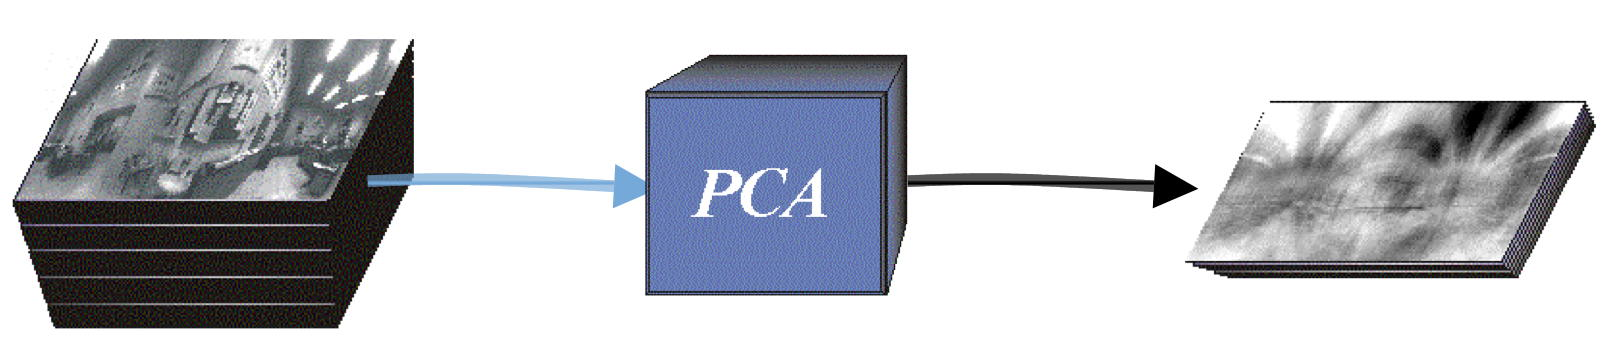
\includegraphics[width=10cm]{pca-sketch}}
\end{frame}

\begin{frame}
  \frametitle{Principal Component Analysis}
  \center{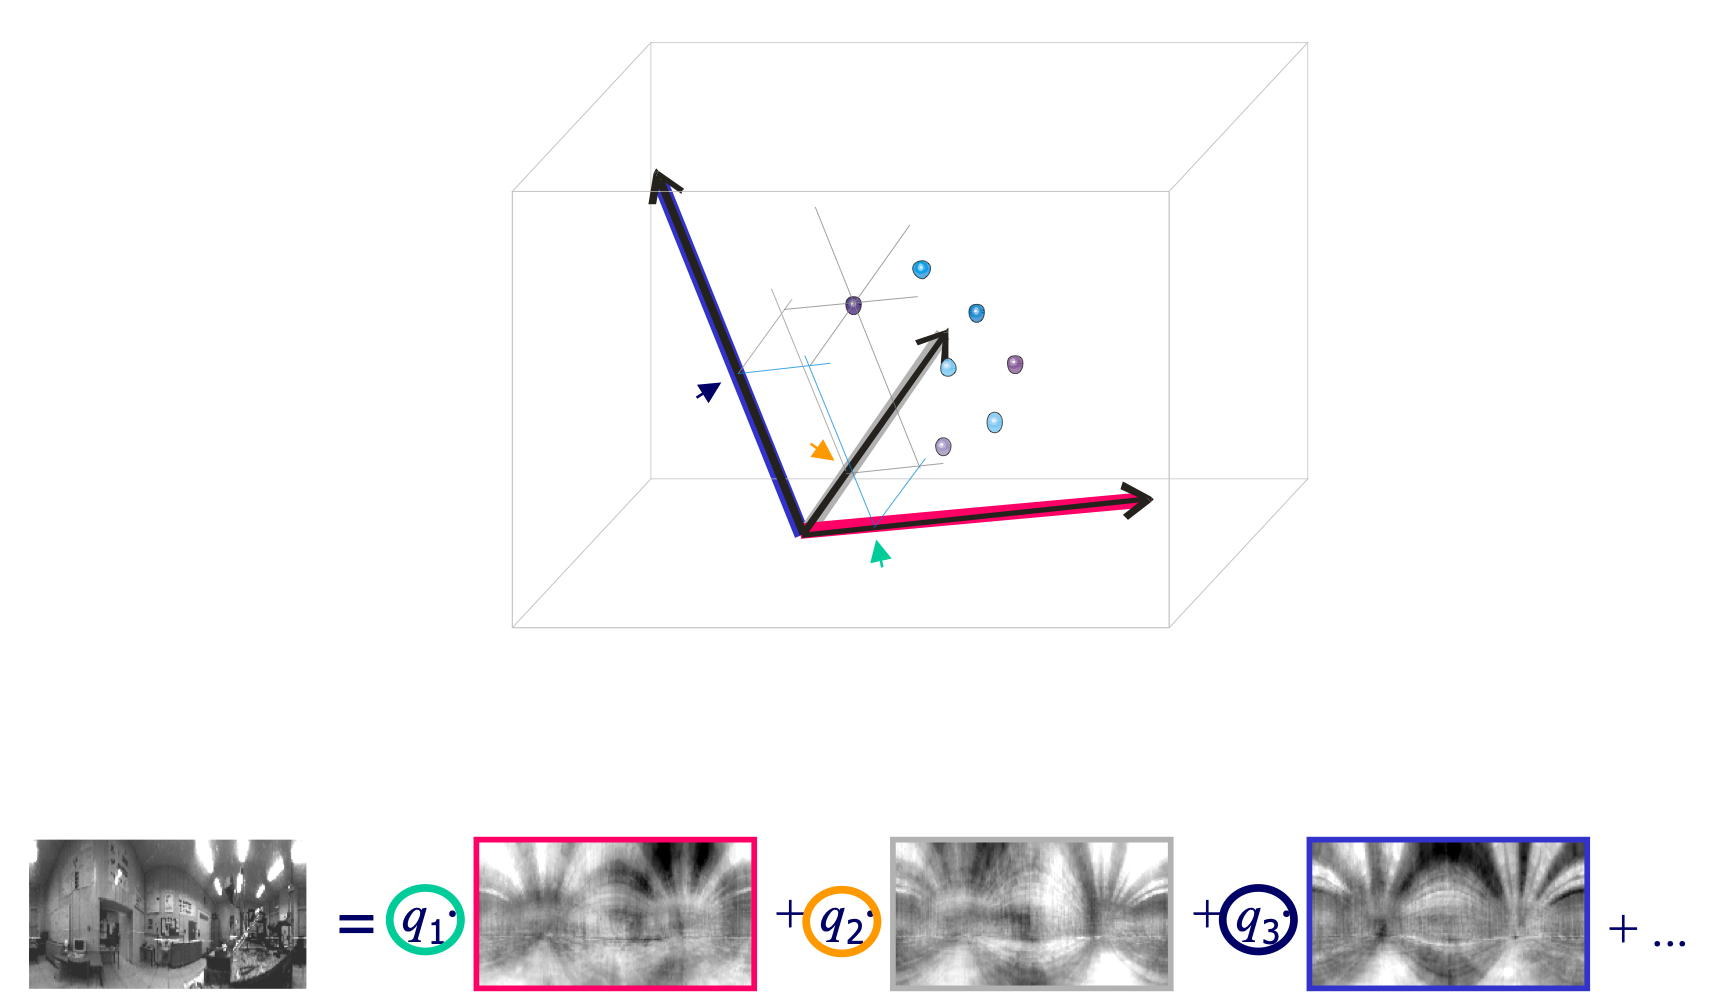
\includegraphics[width=10cm]{pca-composition}}
\end{frame}


\begin{frame}
  \frametitle{PCA Image Representation}
  \center{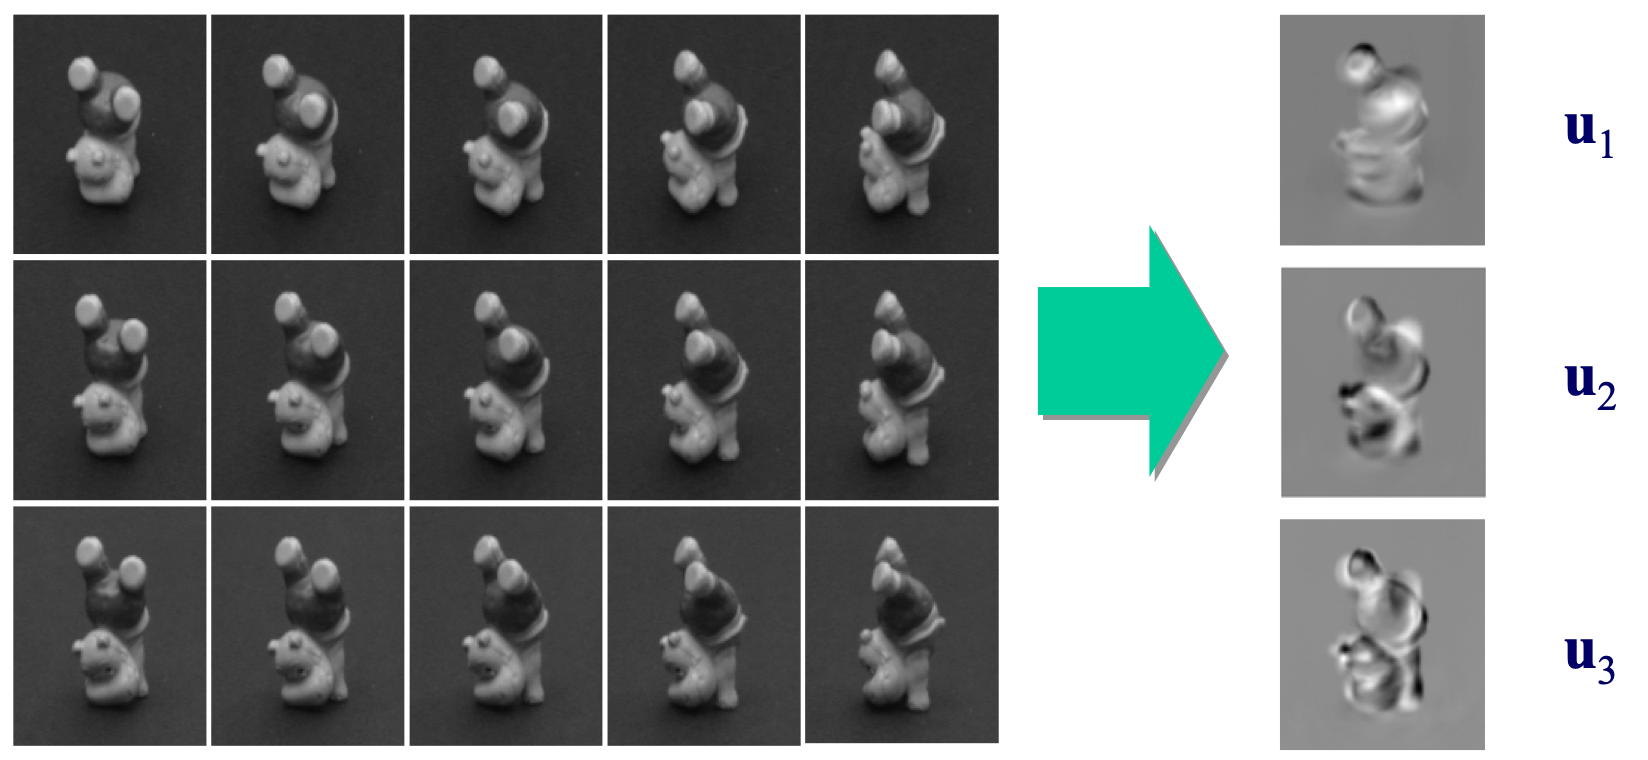
\includegraphics[width=10cm]{pca-image-representation}}
\end{frame}

\begin{frame}
  \frametitle{Properties of PCA}
  \begin{itemize}
  \item Any point $x_i$ can be projected to an appropriate point $q_i$ by
    \[ q_i = U^T (x_i - \mu ) \]
  \item and conversely
    \[ U q_i + \mu = x_i \]
  \end{itemize}
  \centerline{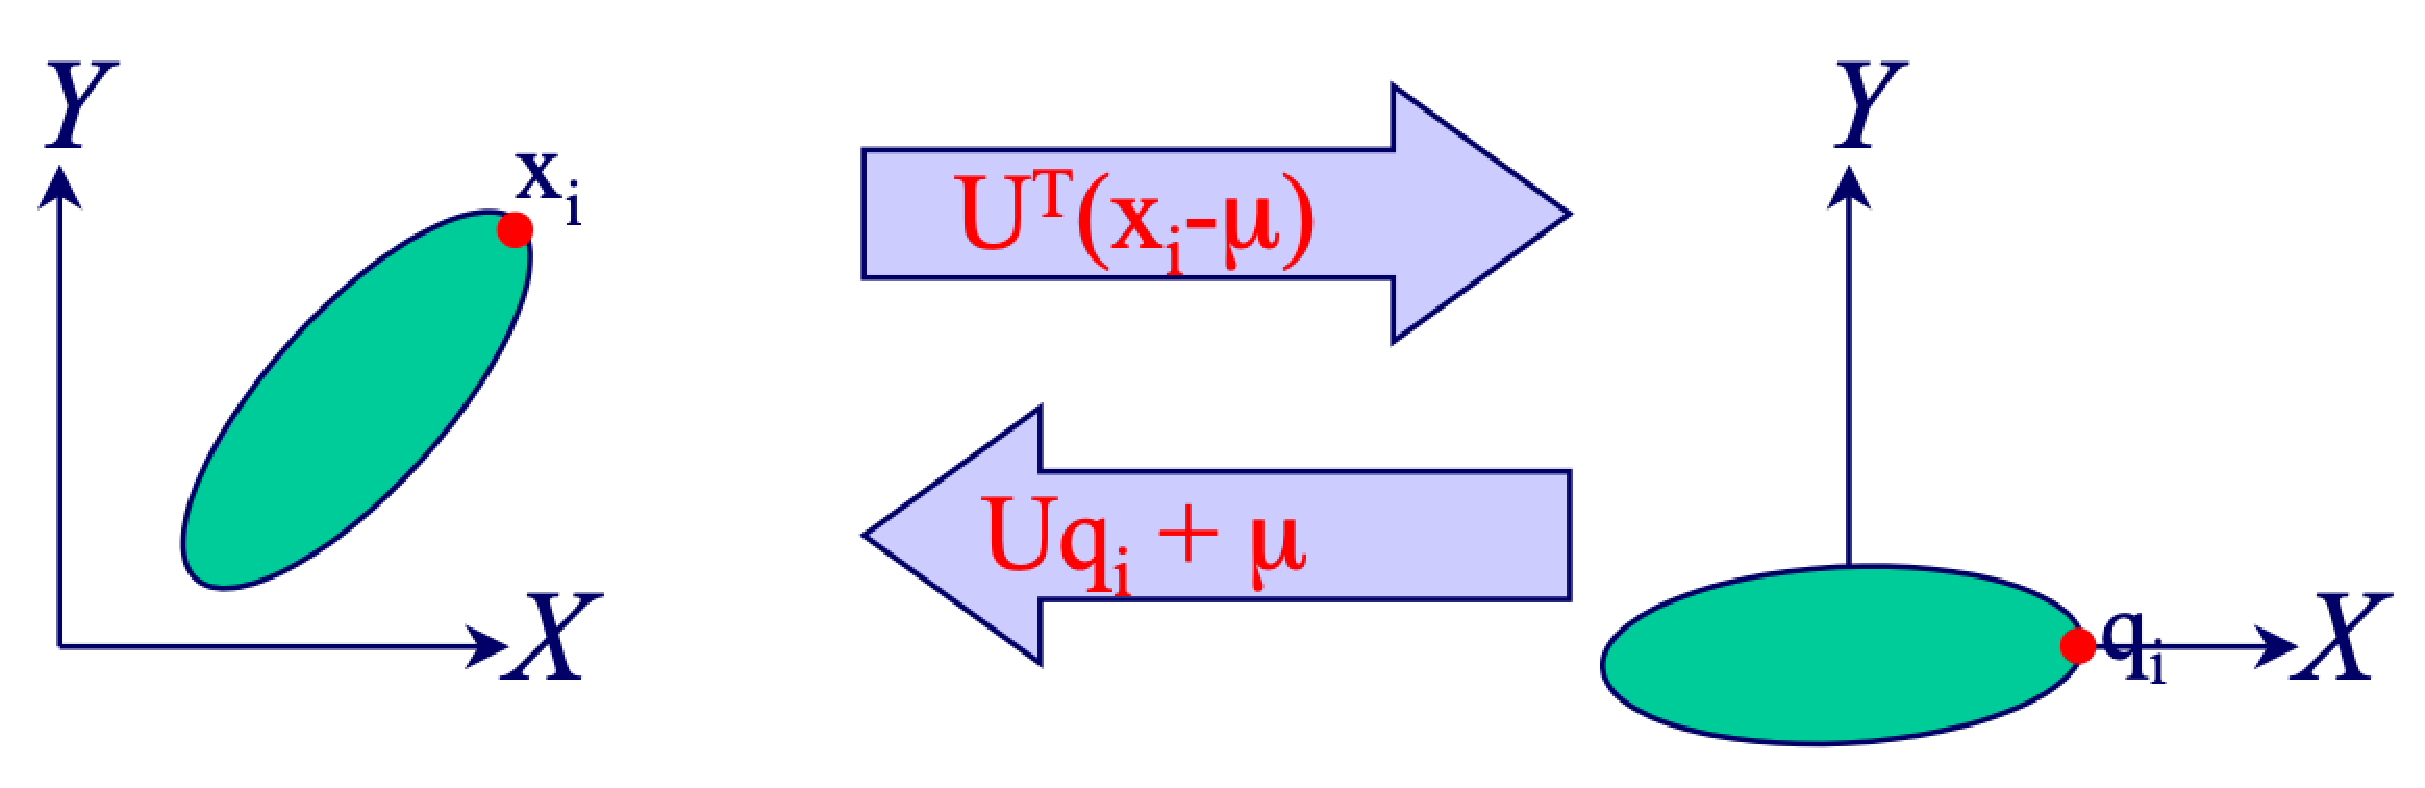
\includegraphics[height=2.5cm]{pca-properties}}
\end{frame}

\begin{frame}
  \frametitle{Properties of PCA}
  \begin{itemize}
  \item It can be shown the MSE between $x_i$ and its reconstruction
    using m eigenvectors is given by
    \[
      \sum_{j=1}^N \lambda_j - \sum_{j=1}^m \lambda_j = \sum_{j=m+1}^N \lambda_j
    \]
  \item PCA minimizes the reconstruction error
  \item PCA maximizes the variance of projection
  \item Find a ``natural'' coordinate system for the sample data
  \end{itemize}
\end{frame}

\begin{frame}
  \frametitle{PCA for visual recognition and pose estimation}
  \begin{itemize}
  \item Objects/images are represented as coordinates in an m-dimension space
  \item An example
    \begin{itemize}
    \item 3D space with points representing objects on a manifold of
      parametric eigenspace such as orientation, pose, illumination,
      ...
    \end{itemize}
  \end{itemize}
  \centerline{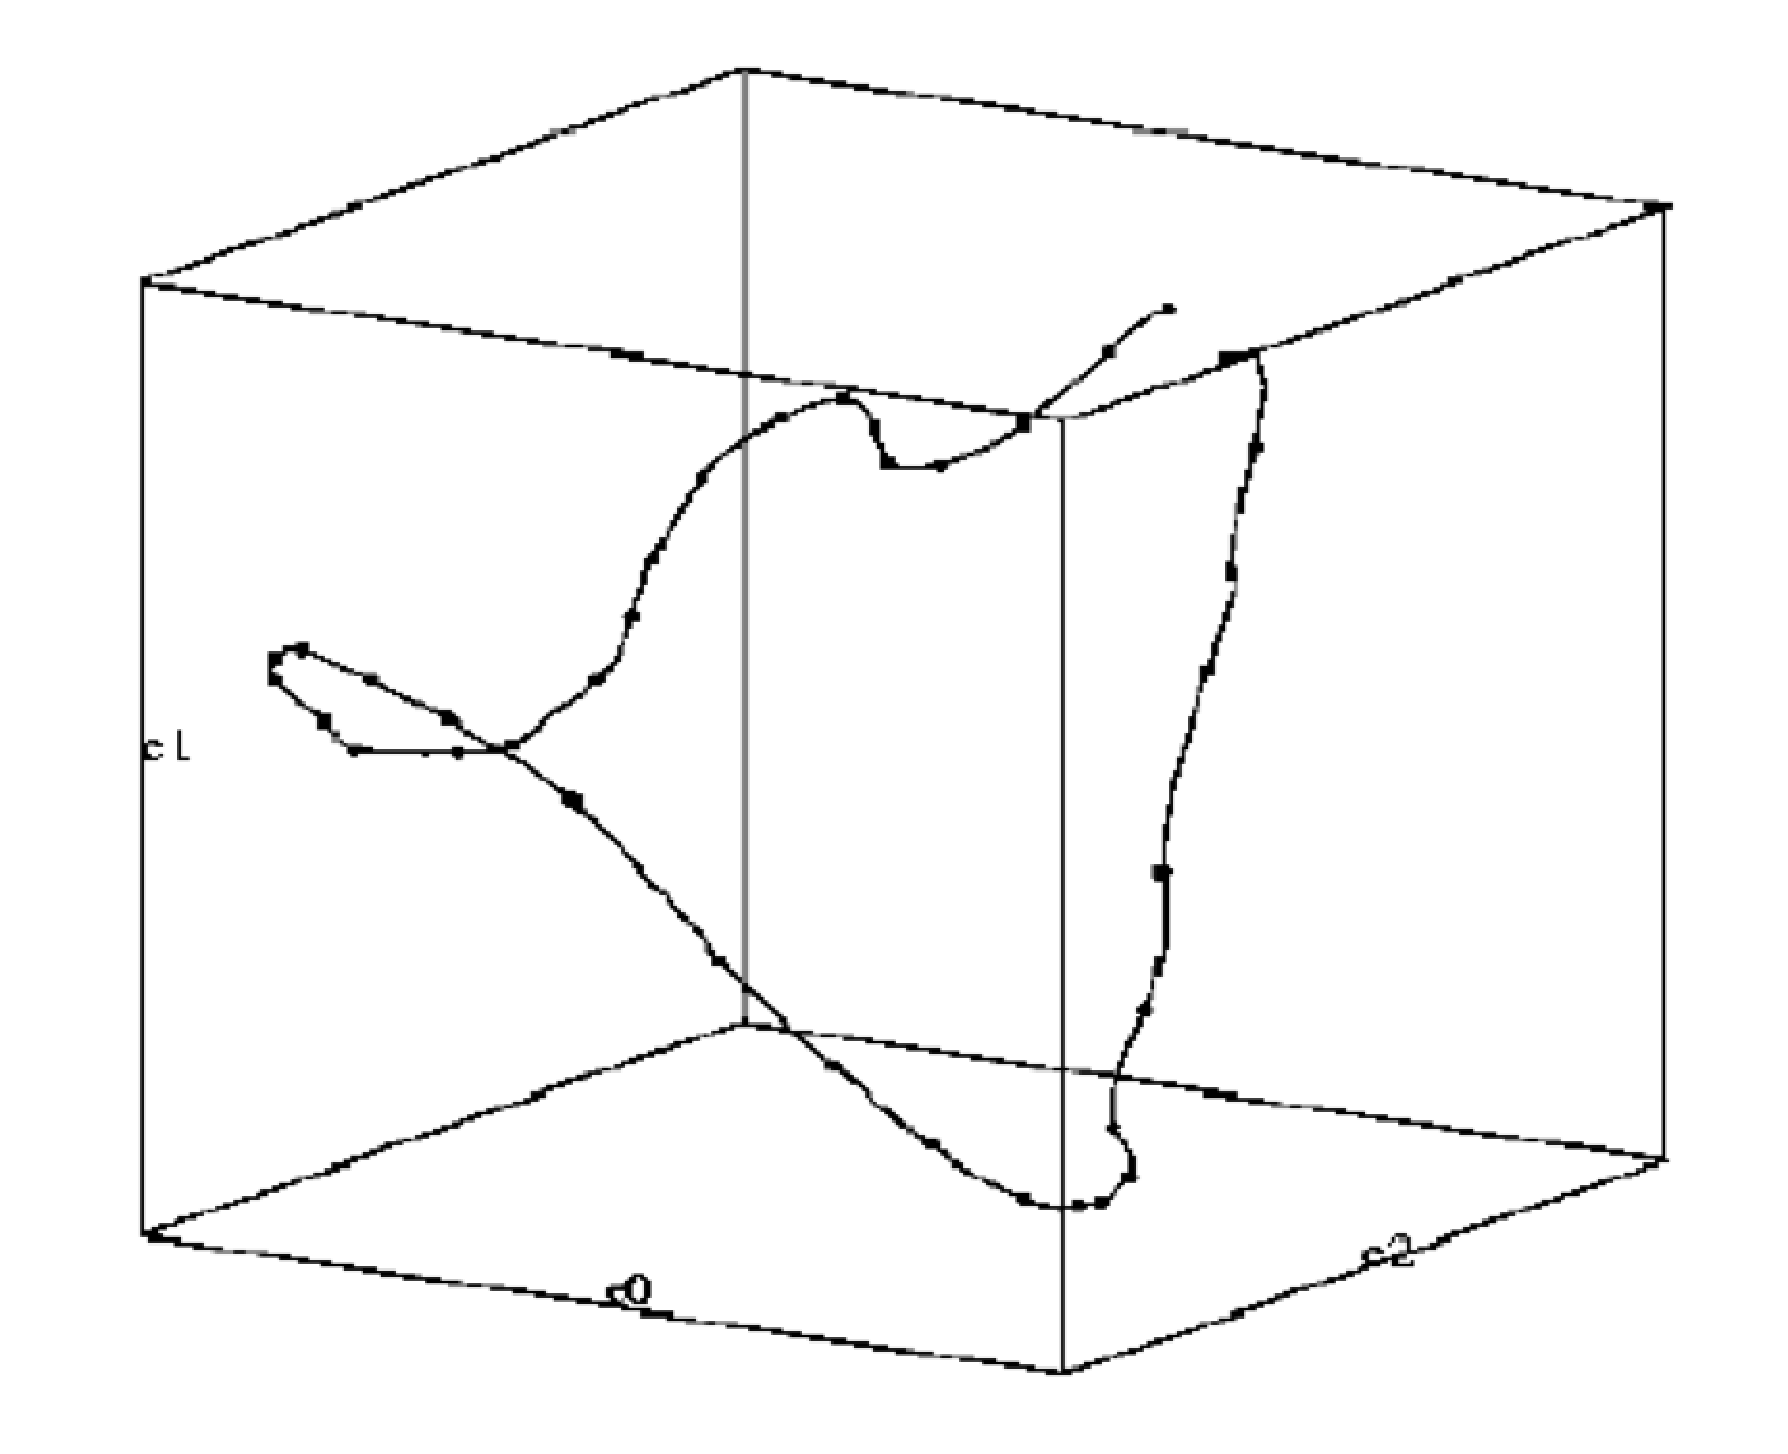
\includegraphics[height=4cm]{pca-eigen-manifold}}
\end{frame}

\begin{frame}
  \frametitle{PCA for visual recognition and pose estimation}
  \begin{itemize}
  \item Calculate coefficients
  \item Search for nearest point on manifold
  \item Point determines / interpolates object and/or pose
  \end{itemize}
  \centerline{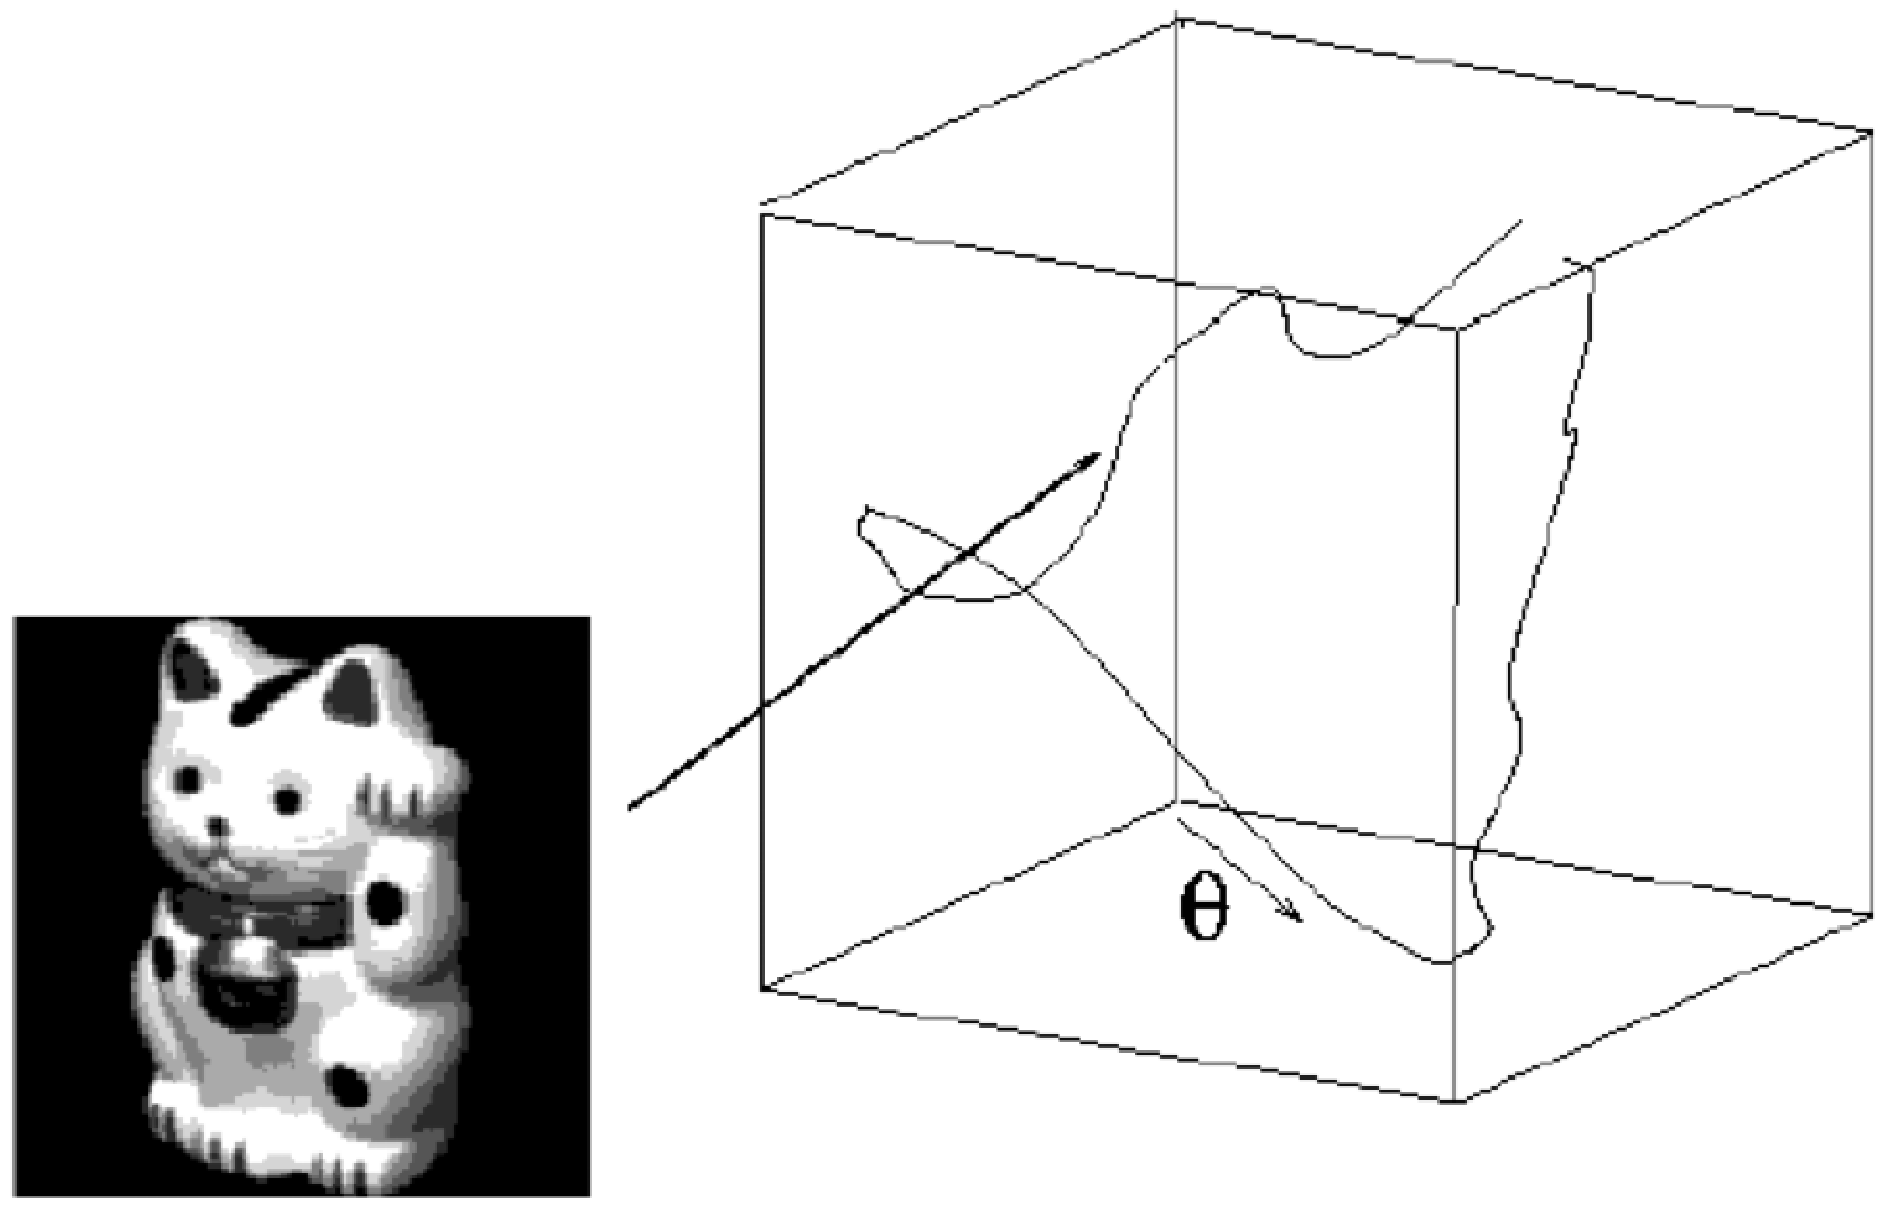
\includegraphics[height=4cm]{pca-manifold-sample}}
\end{frame}

\begin{frame}
  \frametitle{Coefficient calculation}
  \begin{itemize}
  \item To recover $a_i$ the image is projected into the eigenspace
    \centerline{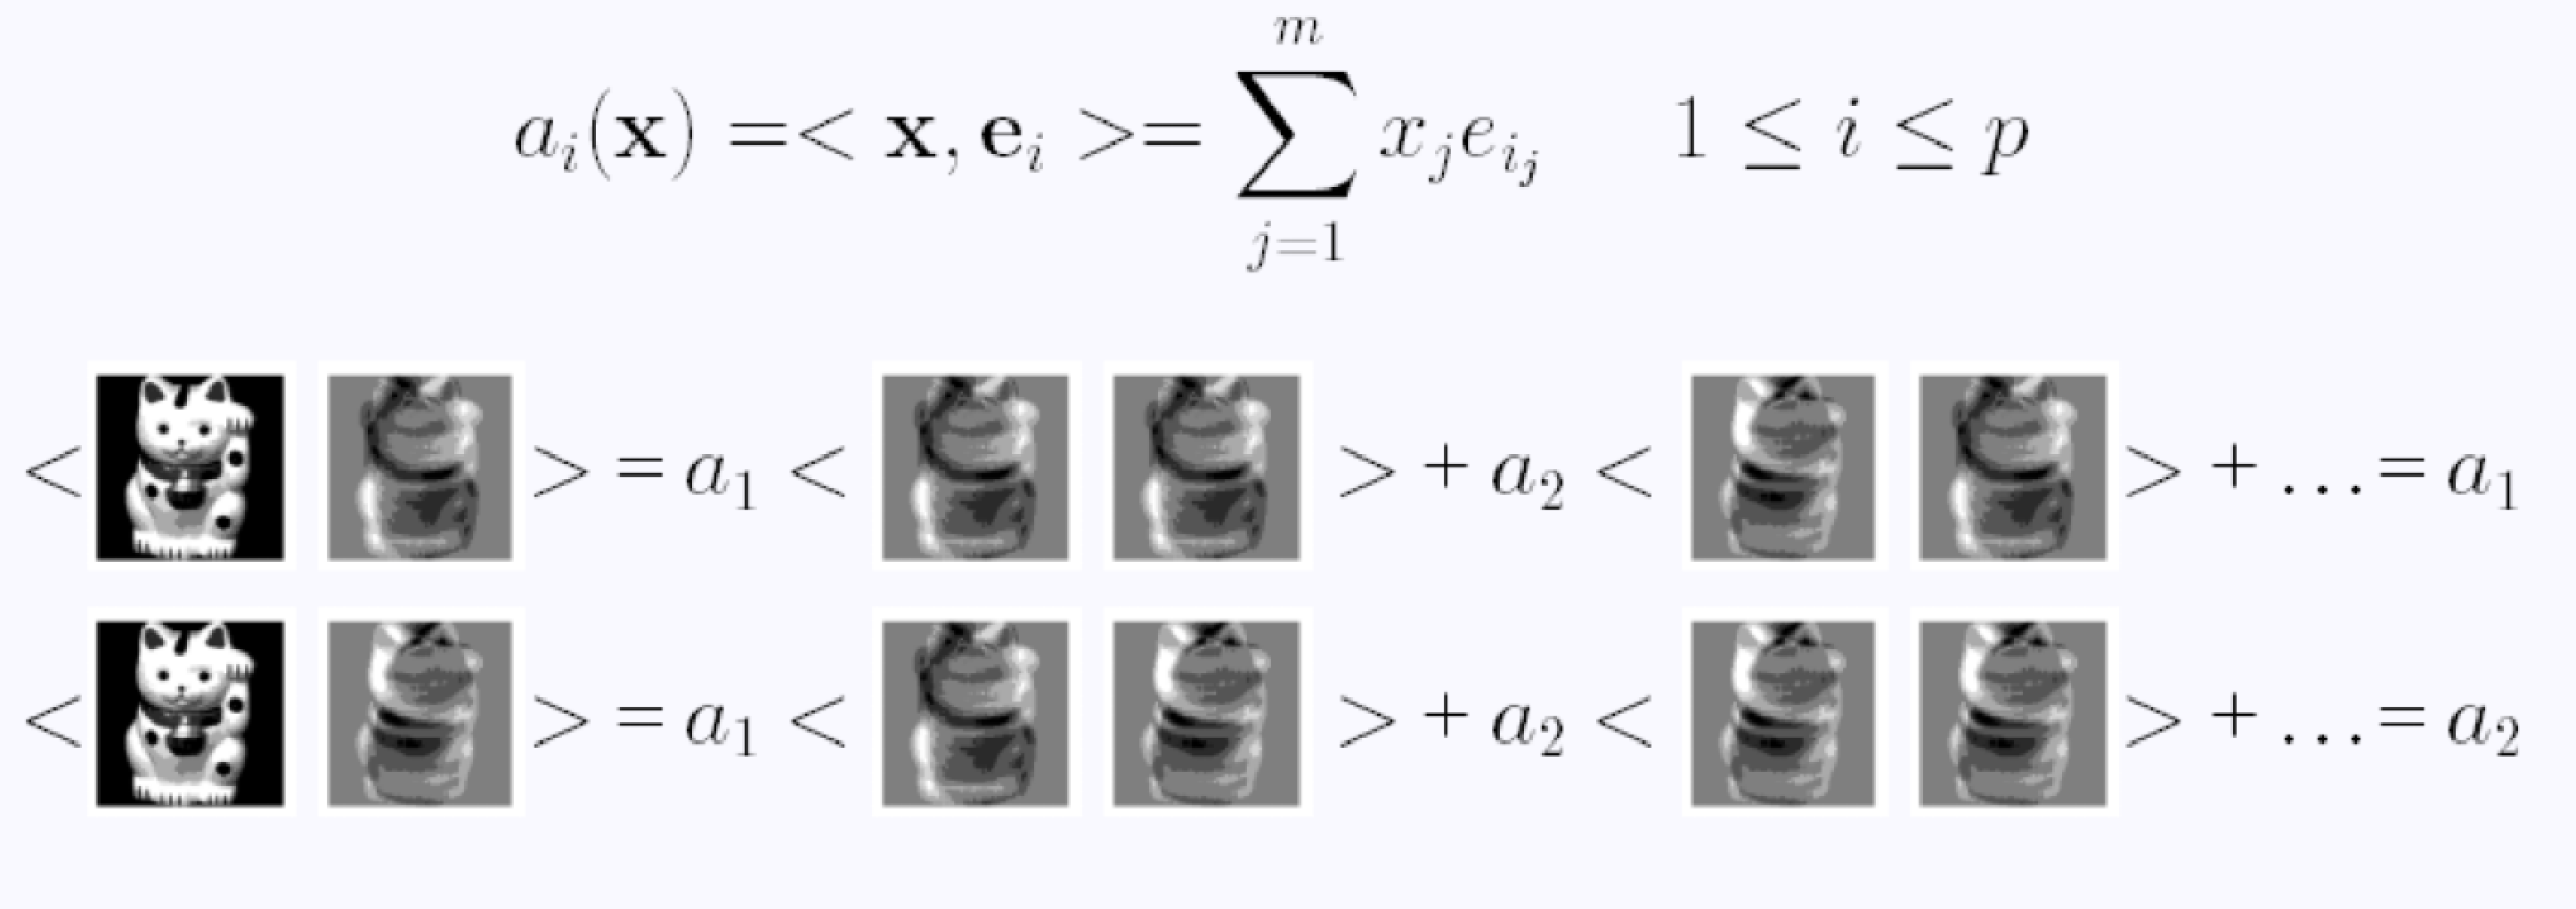
\includegraphics[height=3cm]{pca-calculation}}
  \item Complete image $x_i$ is required to calculate $a_i$
  \item Corresponds to a least square solution
  \end{itemize}
\end{frame}

\section{Linear Discriminative Analysis}
\label{sec:lda}

\begin{frame}
  \frametitle{Linear Discriminate Analysis}
  \begin{itemize}
  \item PCA minimizes the projection error
    \centerline{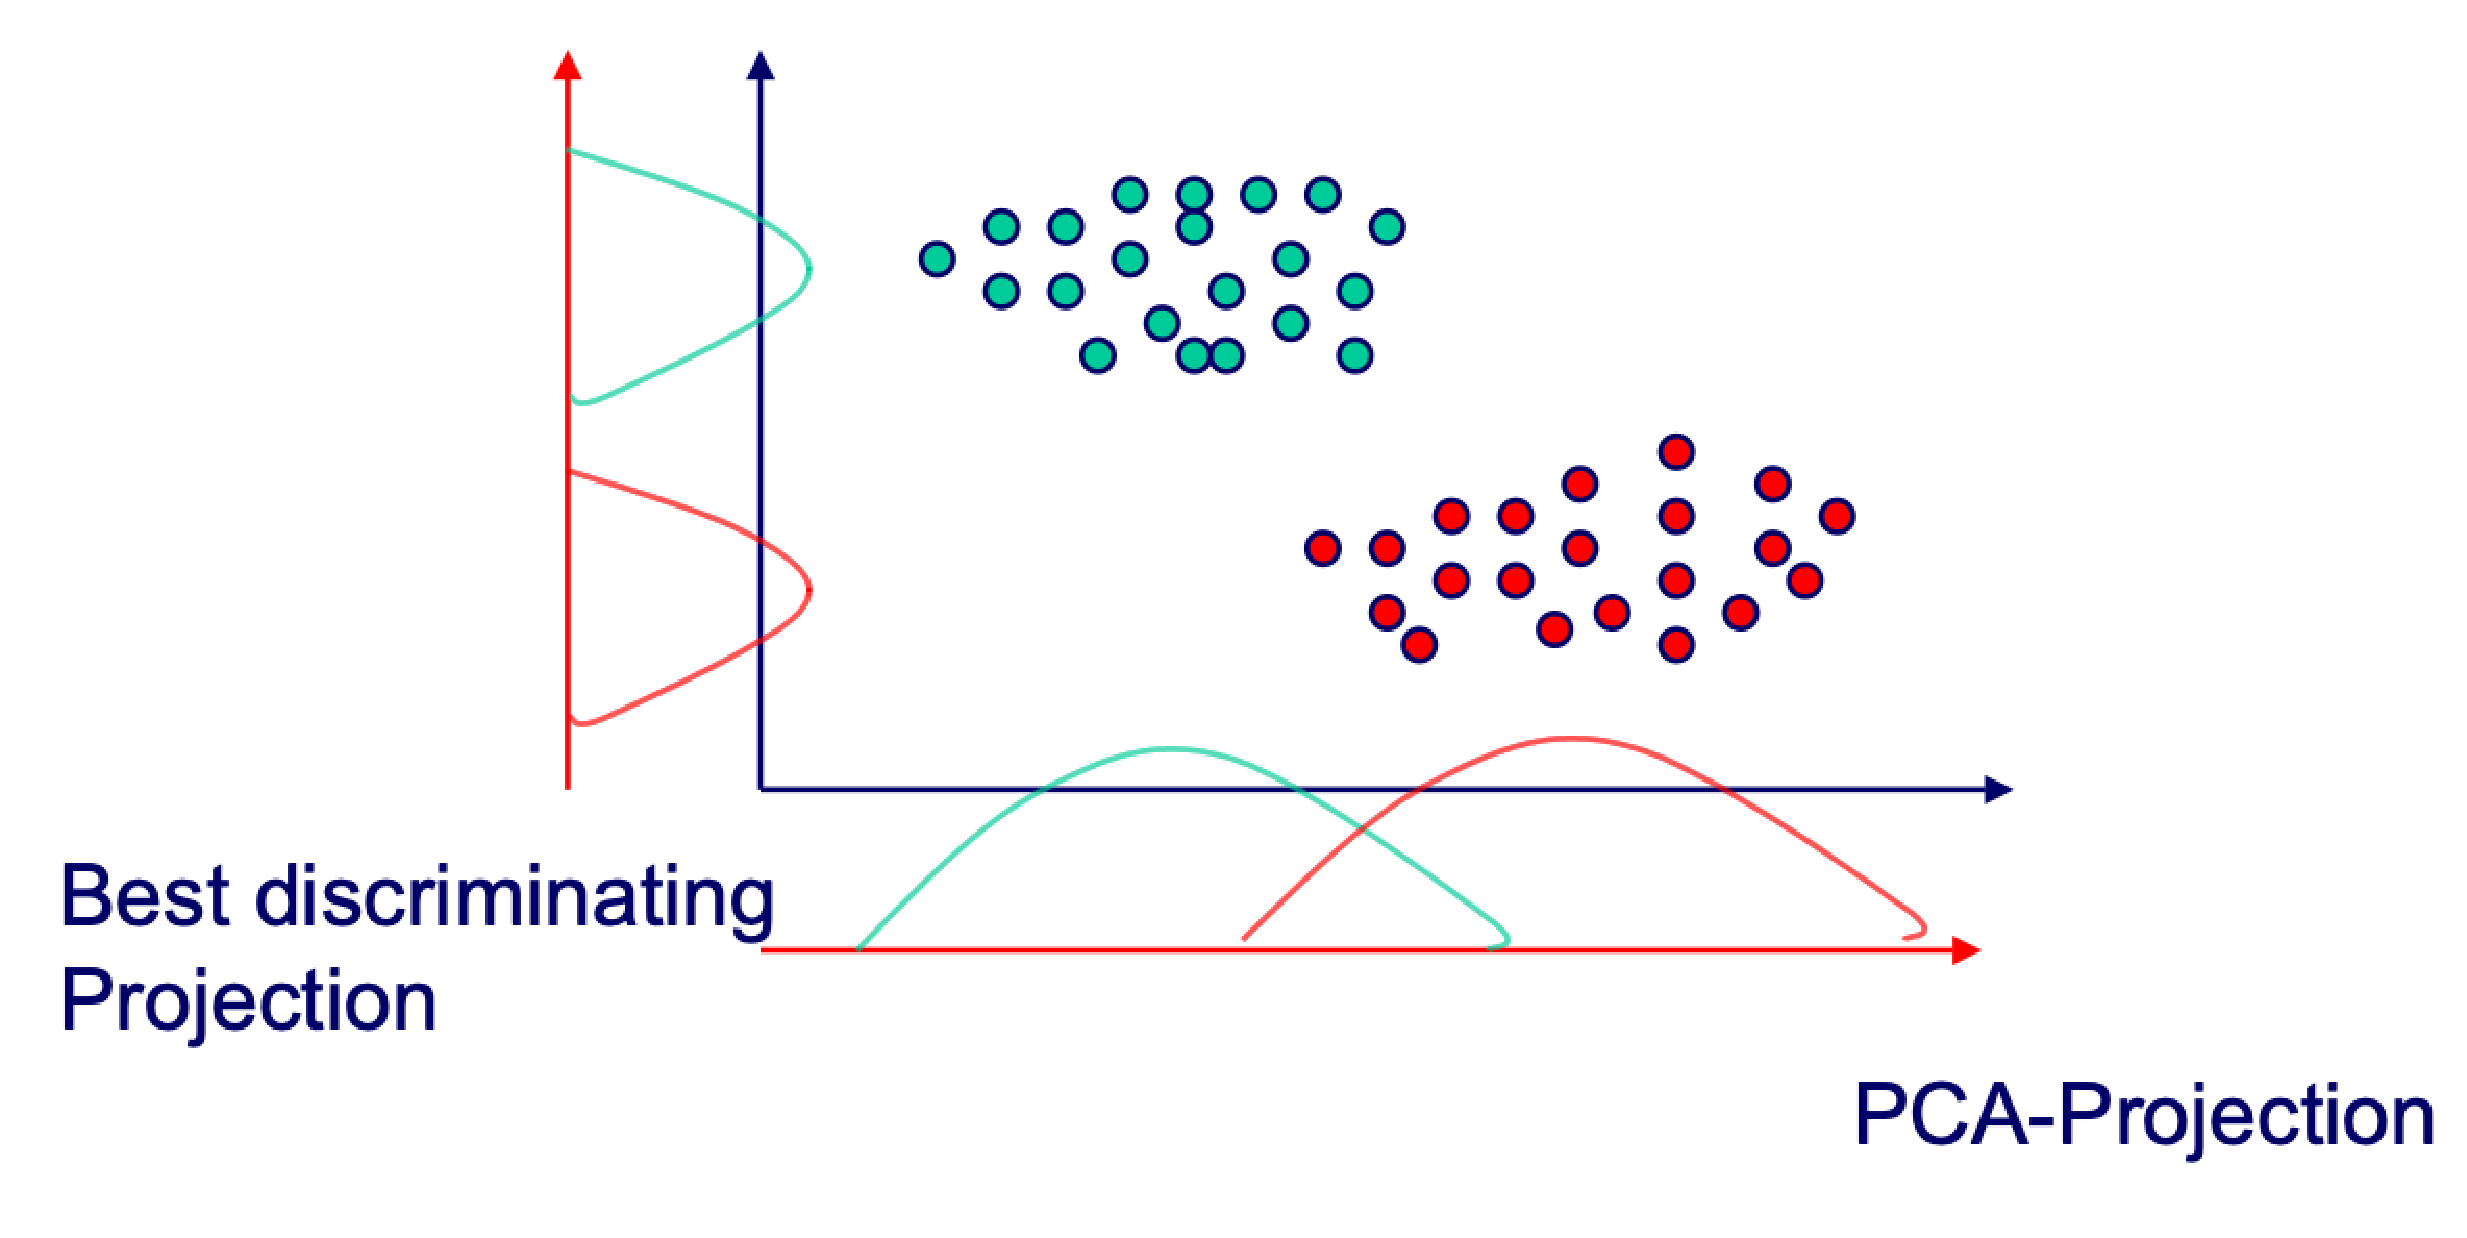
\includegraphics[height=4cm]{pca-projection}}
  \item PCA is unsupervised -- no class information is used
  \item Discriminating information may be used
  \end{itemize}
\end{frame}

\begin{frame}
  \frametitle{Linear Discriminate Analysis}
  \begin{itemize}
  \item For LDA would would like to
    \begin{itemize}
    \item Maximize distance between classes
    \item Minimize distance within classes
    \end{itemize}
  \item Fisher linear discriminant
    \[
      \rho (W) = \frac{W^T S_B W}{W^T S_W W}
    \]
  \end{itemize}
\end{frame}

\begin{frame}
  \frametitle{LDA: Problem Formulation}
  \begin{itemize}
  \item n sample images: \hfill $ \{ x_1, \ldots, x_n \} $
  \item c classes: \hfill $ \{ \chi_1, \ldots, \chi_c \} $
  \item Average of each class: \hfill  $ \mu_i = \frac{1}{n_i} \sum_{x_k \in \chi_i} x_k $
  \item Total average: \hfill $\mu = \frac{1}{n} \sum_{k=1}^N x_k $
  \end{itemize}
\end{frame}

\begin{frame}
  \frametitle{LDA: Practice}
  \begin{itemize}
  \item Scatter of class i: \hfill $ S_i = \sum_{x_k \in \chi_i} (x_k - \mu_i)(x_k - mu_i)^T$
  \item Within class scatter: \hfill $ S_W = \sum_{i=1}^c S_i$
  \item Between class scatter: \hfill $S_B = \sum_{i=1}^c |\chi_i|(\mu_i - \mu)(\mu_i - \mu)^T$
  \item Total scatter: \hfill $S_T = S_W + S_B$
  \end{itemize}  
\end{frame}

\begin{frame}
  \frametitle{LDA: Practice}
  \begin{itemize}
  \item After projection: $ y_k = W^T x_k $
    \begin{itemize}
    \item Between class scatter of y: $\tilde{S}_B = W^T S_B W$
    \item Within class scatter of y: $\tilde{S}_W = W^T S_W W$
    \end{itemize}
  \end{itemize}
\end{frame}

\begin{frame}
  \frametitle{LDA Projection}
  \centerline{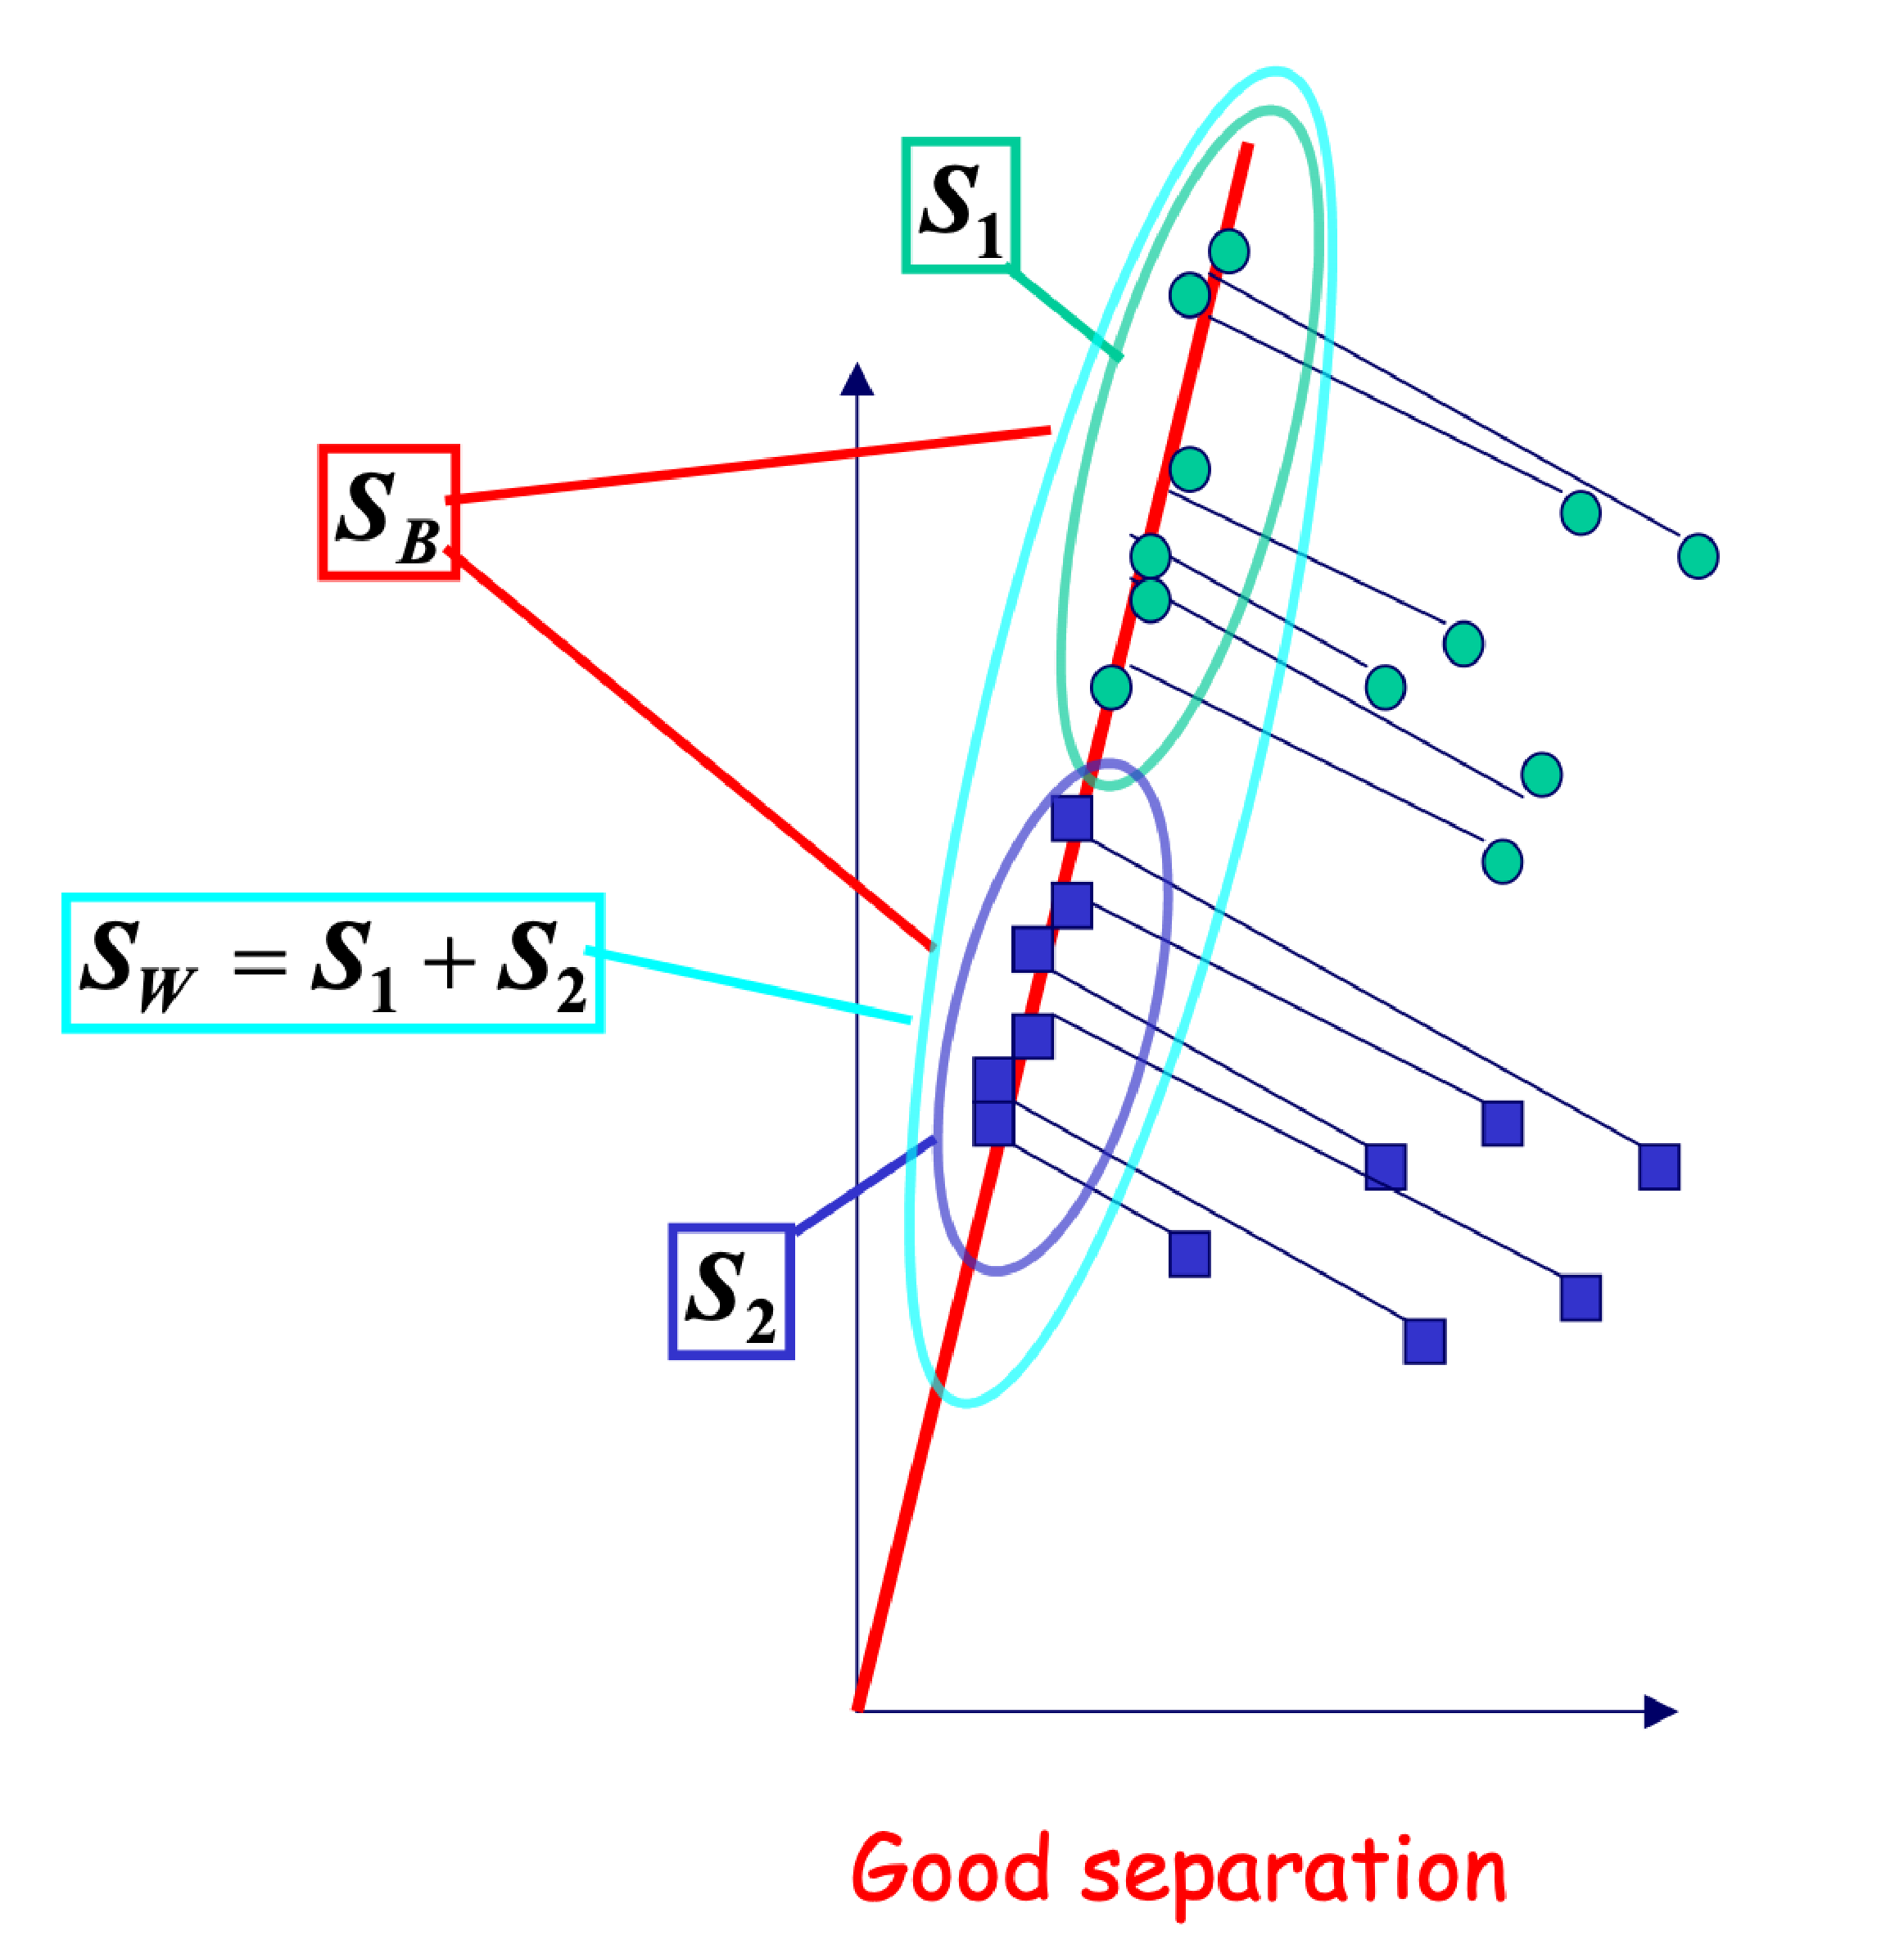
\includegraphics[height=6cm]{lda-projection}}
\end{frame}

\begin{frame}
  \frametitle{LDA characteristics}
  \begin{itemize}
  \item Maximization of
    \[
      \rho (W) = \frac{W^T S_B W}{W^T S_W W}
    \]
  \item given by solution of generalized eigenvalue problem
    \[
      S_B W = \lambda S_W W
    \]
  \item The the c-class case we obtain c-1 projections as the largest eigenvalue of
    \[
      S_B W_i = \lambda S_W W_i
    \]
  \end{itemize}
\end{frame}

\begin{frame}
  \frametitle{LDA in the wild}
  \begin{itemize}
  \item How does one calculate LDA for high-dimensional images? 
  \item Problem: $S_W$ is always singular
    \begin{itemize}
    \item Number of pixels in an image is larger than number of images in training set
    \end{itemize}
  \item Fisherfaces example: reduce dimensionality by doing a PCA first and then LDA
  \item Simultaneous diagonalization of $S_W$ and $S_B$
  \end{itemize}
\end{frame}

\begin{frame}
  \frametitle{Ficherfaces}
  \begin{itemize}
  \item First published by Belhumeur et al 1997
  \item Reduce dimensionality to n-c with PCA
    \[
      U_{PCA} = \arg \max_U | U^T Q U | = [~u_1 ~ u_2 \ldots ~ u_{n-c} ~]
    \]
  \item Further reduce to c-1 with LDA
    \[
      W_{LDA} = \arg \max_w \frac{| W^T W^T_{pca} S_B W_{pca} W |}{| W^T W^T_{pca} S_W W_{pca} W |} =
      [~ w_1 ~ w_2 ~ \ldots ~ w_{c-1} ~]
    \]
  \item The optimal projection is then
    \[
      W_{opt} = W_{LDA}^T U^T
    \]
  \end{itemize}
\end{frame}


\begin{frame}
  \frametitle{Example Fisherface}
  \begin{itemize}
  \item Example Fisherface of recognition face w/wo glasses (Belhumeur et al, 1997)
  \end{itemize}
  \centerline{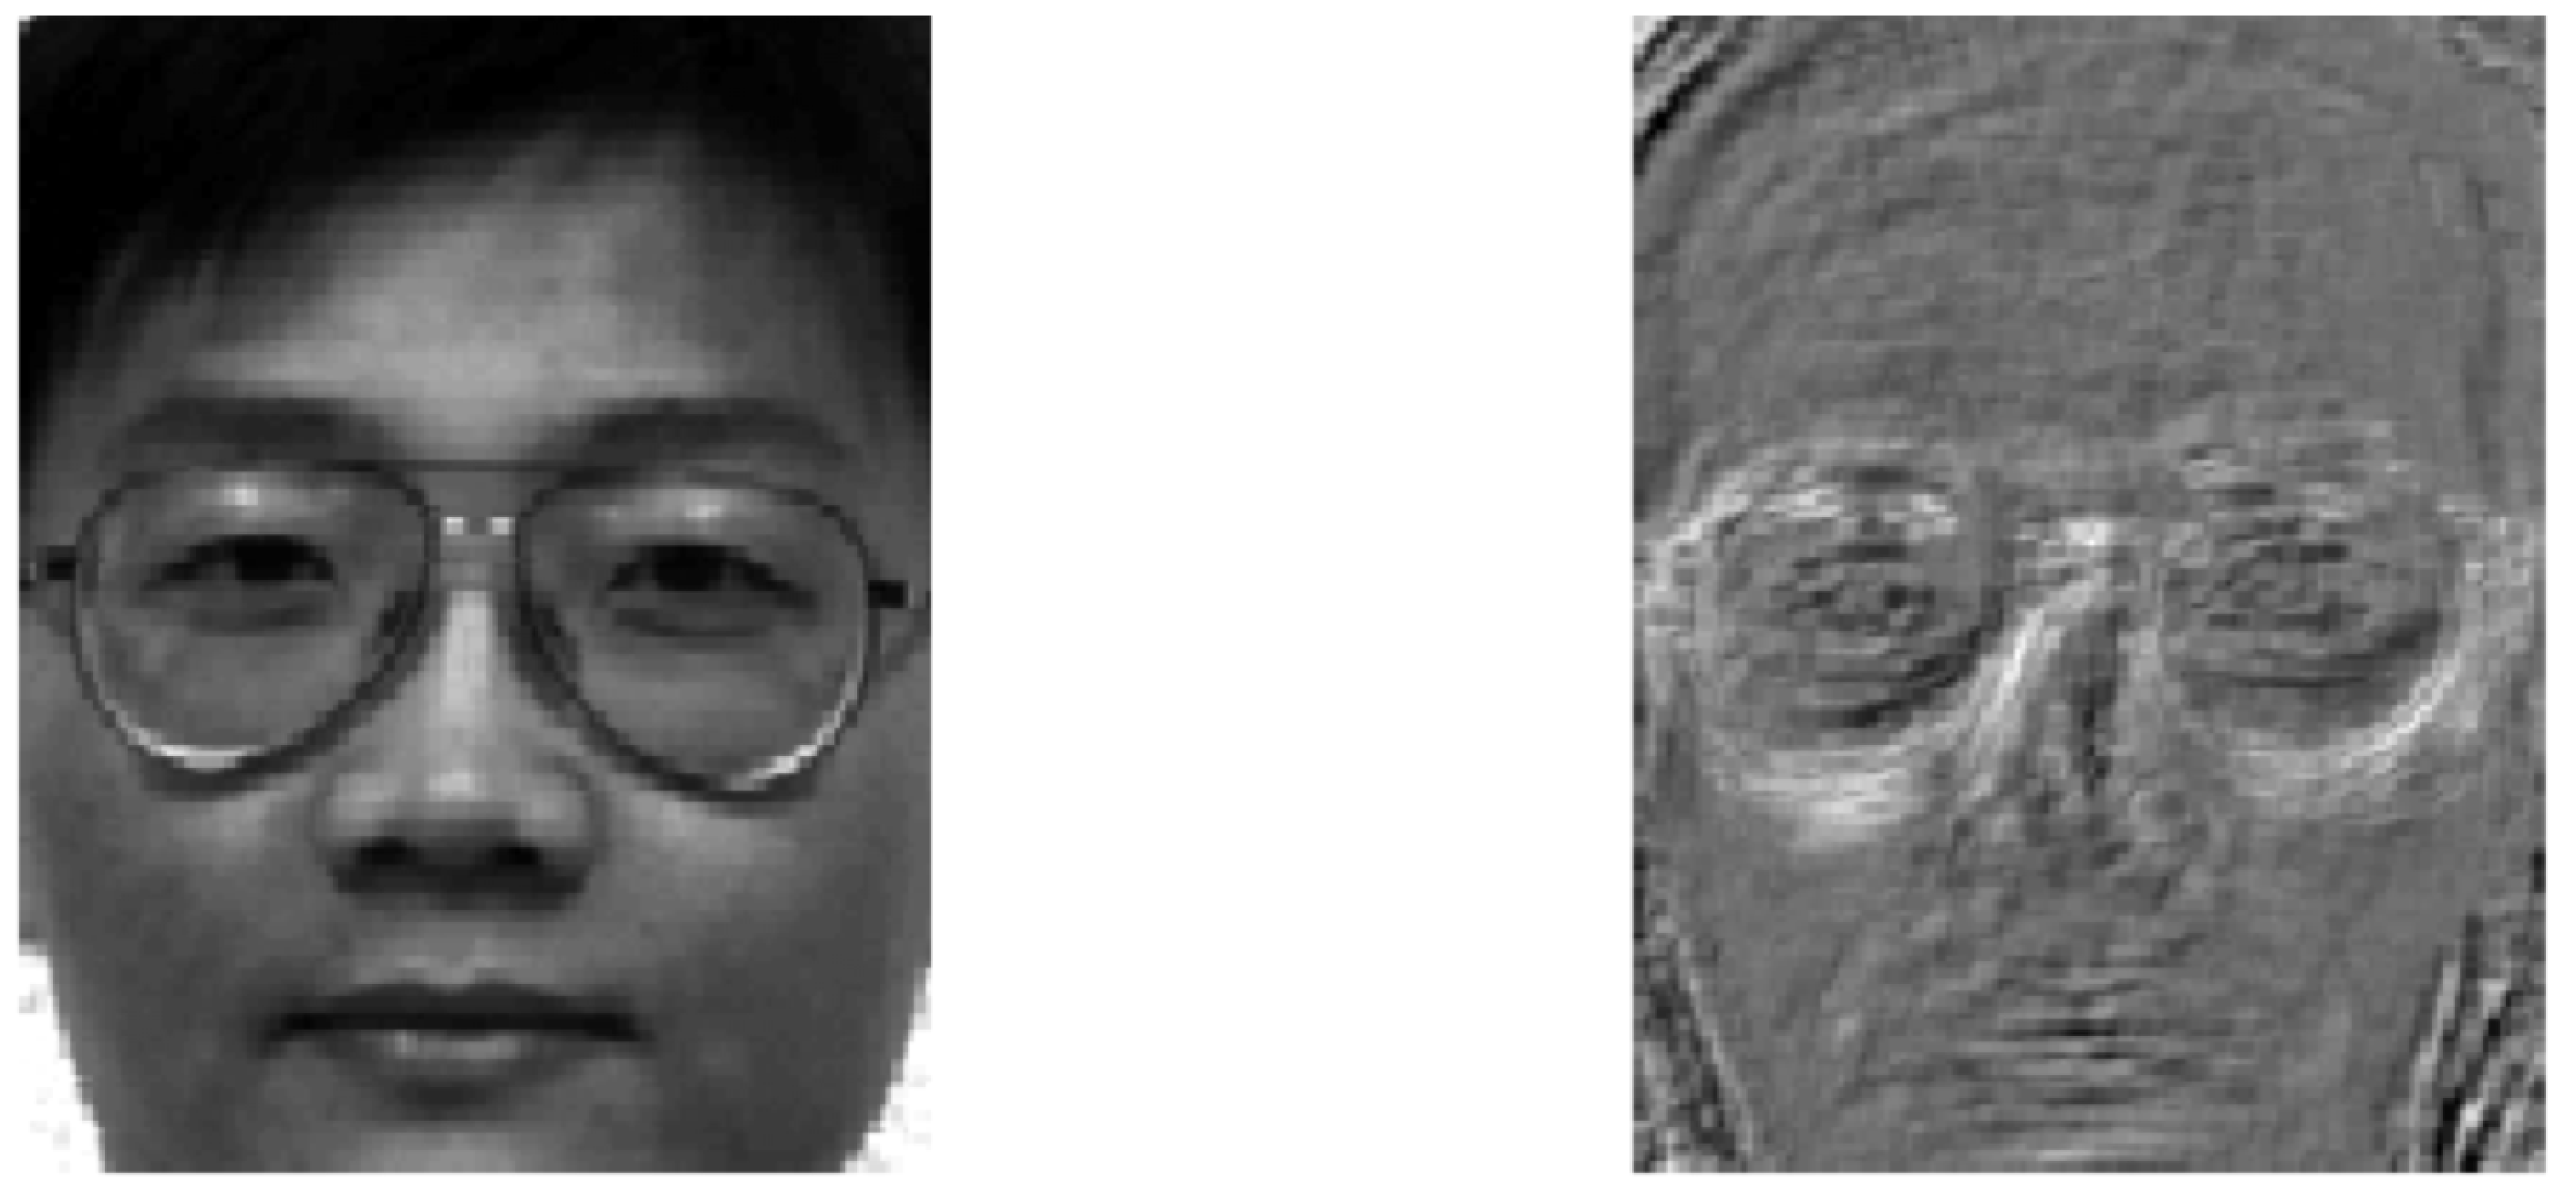
\includegraphics[height=4cm]{fisherface}}
\end{frame}

\begin{frame}
  \frametitle{Fisher example performance}
  \begin{itemize}
  \item Small comparison of face recognition (old data)
    \centerline{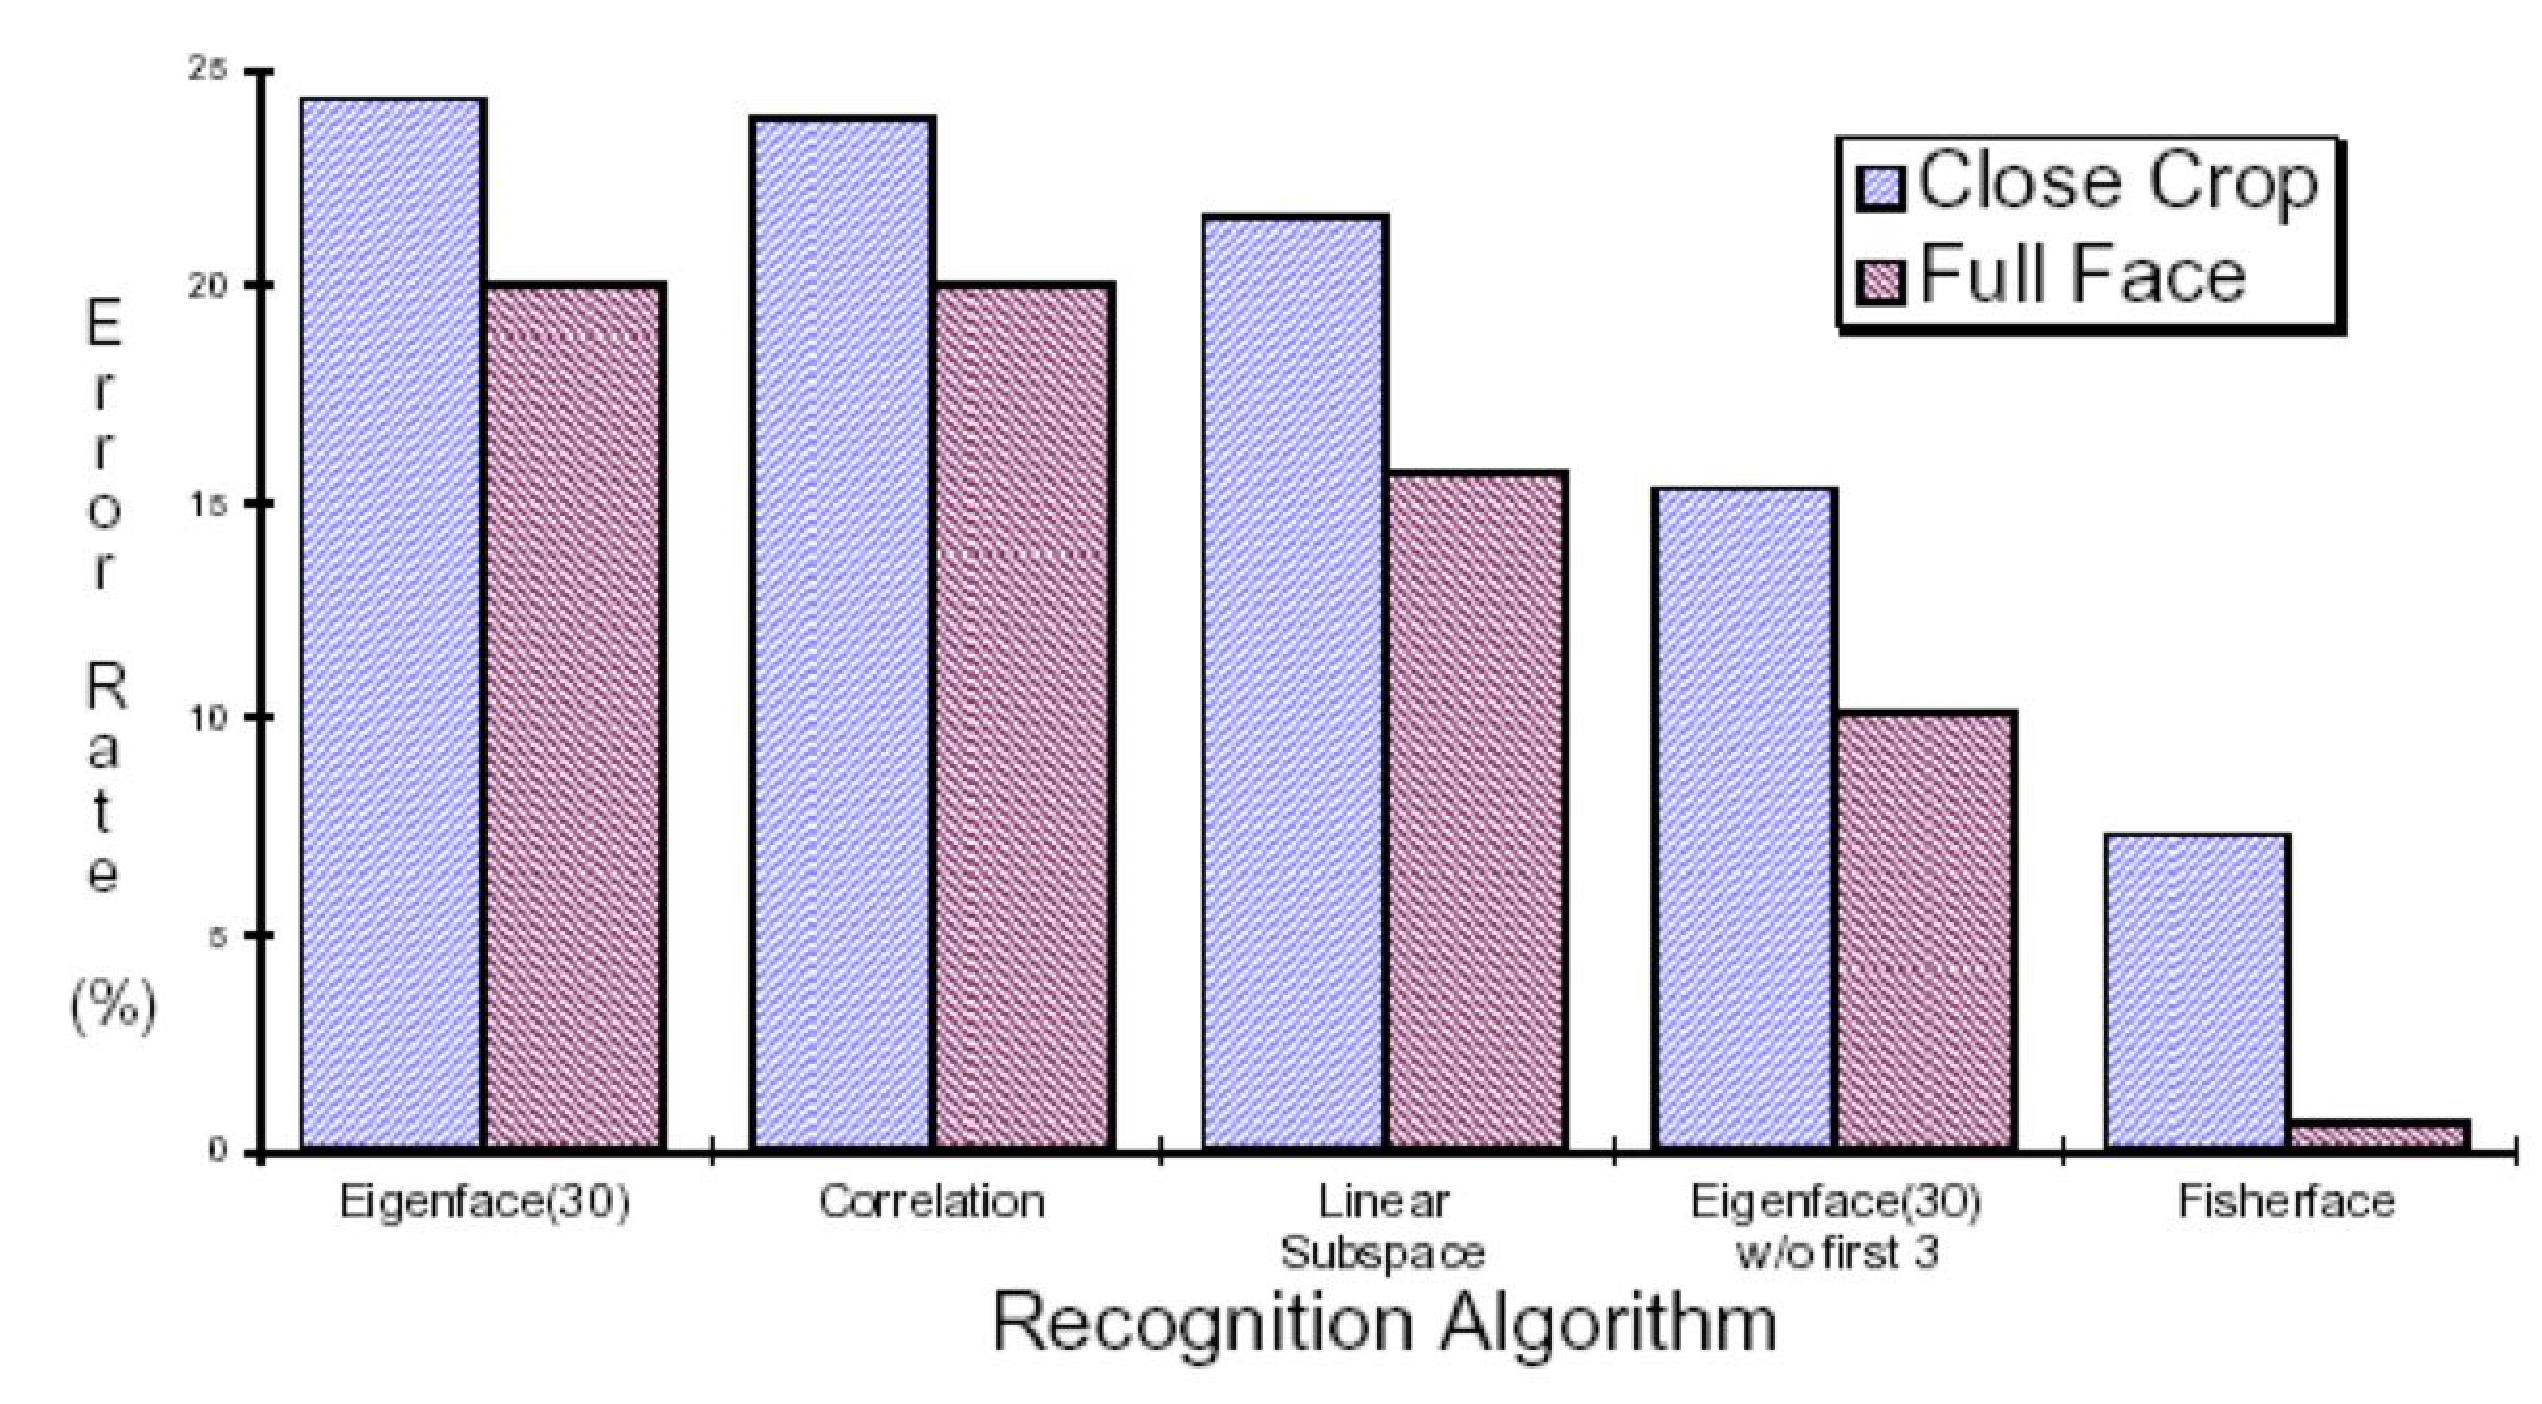
\includegraphics[height=3.5cm]{fisher-performance}}
  \item Significantly better performance than PCA for face recognition
  \item Noise sensitive
  \item Standard large scale Kaggle competitions today score ~97\%
  \end{itemize}
\end{frame}


\section{Canonical Correlation Analysis }
\label{sec:cca}

\begin{frame}
  \frametitle{Canonical Correlation Analysis (CCA)}
  \begin{itemize}
  \item Also supervised method by motivated by regression /
    interpolation tasks such as {\color{red} pose estimation}
  \item CCA related two sets of observations by determining pairs of directions that yield
    maximum correlation between the data sets
  \item Find a pair of directions (canonical factors):
    $ w_x \in R^P ~and ~w_y \in R^q $ so that the correlation of the
    projections $c = w_x^T x$ and $d = w_y^T y$ become maximal
  \end{itemize}
\end{frame}

\begin{frame}
  \frametitle{CCA - the details}
  \[
    \rho = \frac{E[cd]}{\sqrt{E[c^2]~E[d^2]}} =
  \]
  \[
    \frac{E[w_x^T x ~ y^t w_y]}{\sqrt{ E[ w_x^T x ~x^T w_x ] E[ w_y^T y ~y^t w_y ]}} =
  \]
  \[
    \frac{w_x^T C_{xy} w_y}{\sqrt{w_x^T C_{xx} w_x w_y^T C_{yy} w_y}}
  \]
\end{frame}

\begin{frame}
  \frametitle{CCA - computations}
  \begin{itemize}
  \item Finding solutions
    \begin{eqnarray*}
      \label{eq:cca}
      w = \left[ \begin{array}{c} w_x \\ w_y \end{array} \right] &
      A = \left[ \begin{array}{cc} 0 & C_{xy} \\ C_{yx} & 0 \end{array} \right] &
      B = \left[ \begin{array}{cc} C_{xx} & 0 \\ 0 & C_{yy} \end{array} \right] 
    \end{eqnarray*}
  \item Compute the Rayleigh Quotient
    \[
      r = \frac{w^T A w}{w^T B w}
    \]
  \item Think of it as a generalized eigenvalue problem
    \[
      A w = \mu B w
    \]
  \end{itemize}
\end{frame}

\begin{frame}
  \frametitle{CCA for images}
  \begin{itemize}
  \item Same challenge as for LDA
  \item Computational analysis based on SVD
    \begin{eqnarray*}
      \label{eq:cca2}
      A = C_{xx}^{-\frac{1}{2}}C_{xy}C_{yy}^{-\frac{1}{2}}\\
      A = U D V^T \\
      w_{xi} = C_{xx}^{-\frac{1}{2}} u_i\\
      w_{yi} = C_{yy}^{-\frac{1}{2}} v_i
    \end{eqnarray*}
  \end{itemize}
\end{frame}

\begin{frame}
  \frametitle{Properties of CCA}
  \begin{itemize}
  \item At most min(p, q, n) CCA factors
  \item Invariant wrt to affine transformations
  \item Orthogonality of the canonical factors
    \begin{eqnarray*}
      w_{xi}^T C_{xx} w_{xj} = 0 \\
      w_{yi}^T C_{yy} w_{yj} = 0 \\
      w_{xi}^T C_{xy} w_{yj} = 0 \\
    \end{eqnarray*}
  \end{itemize}
\end{frame}

\begin{frame}
  \frametitle{CCA Example}
  \begin{itemize}
  \item Parametric eigenspace obtained by PCA for 2 DOF pose space
  \end{itemize}
  \centerline{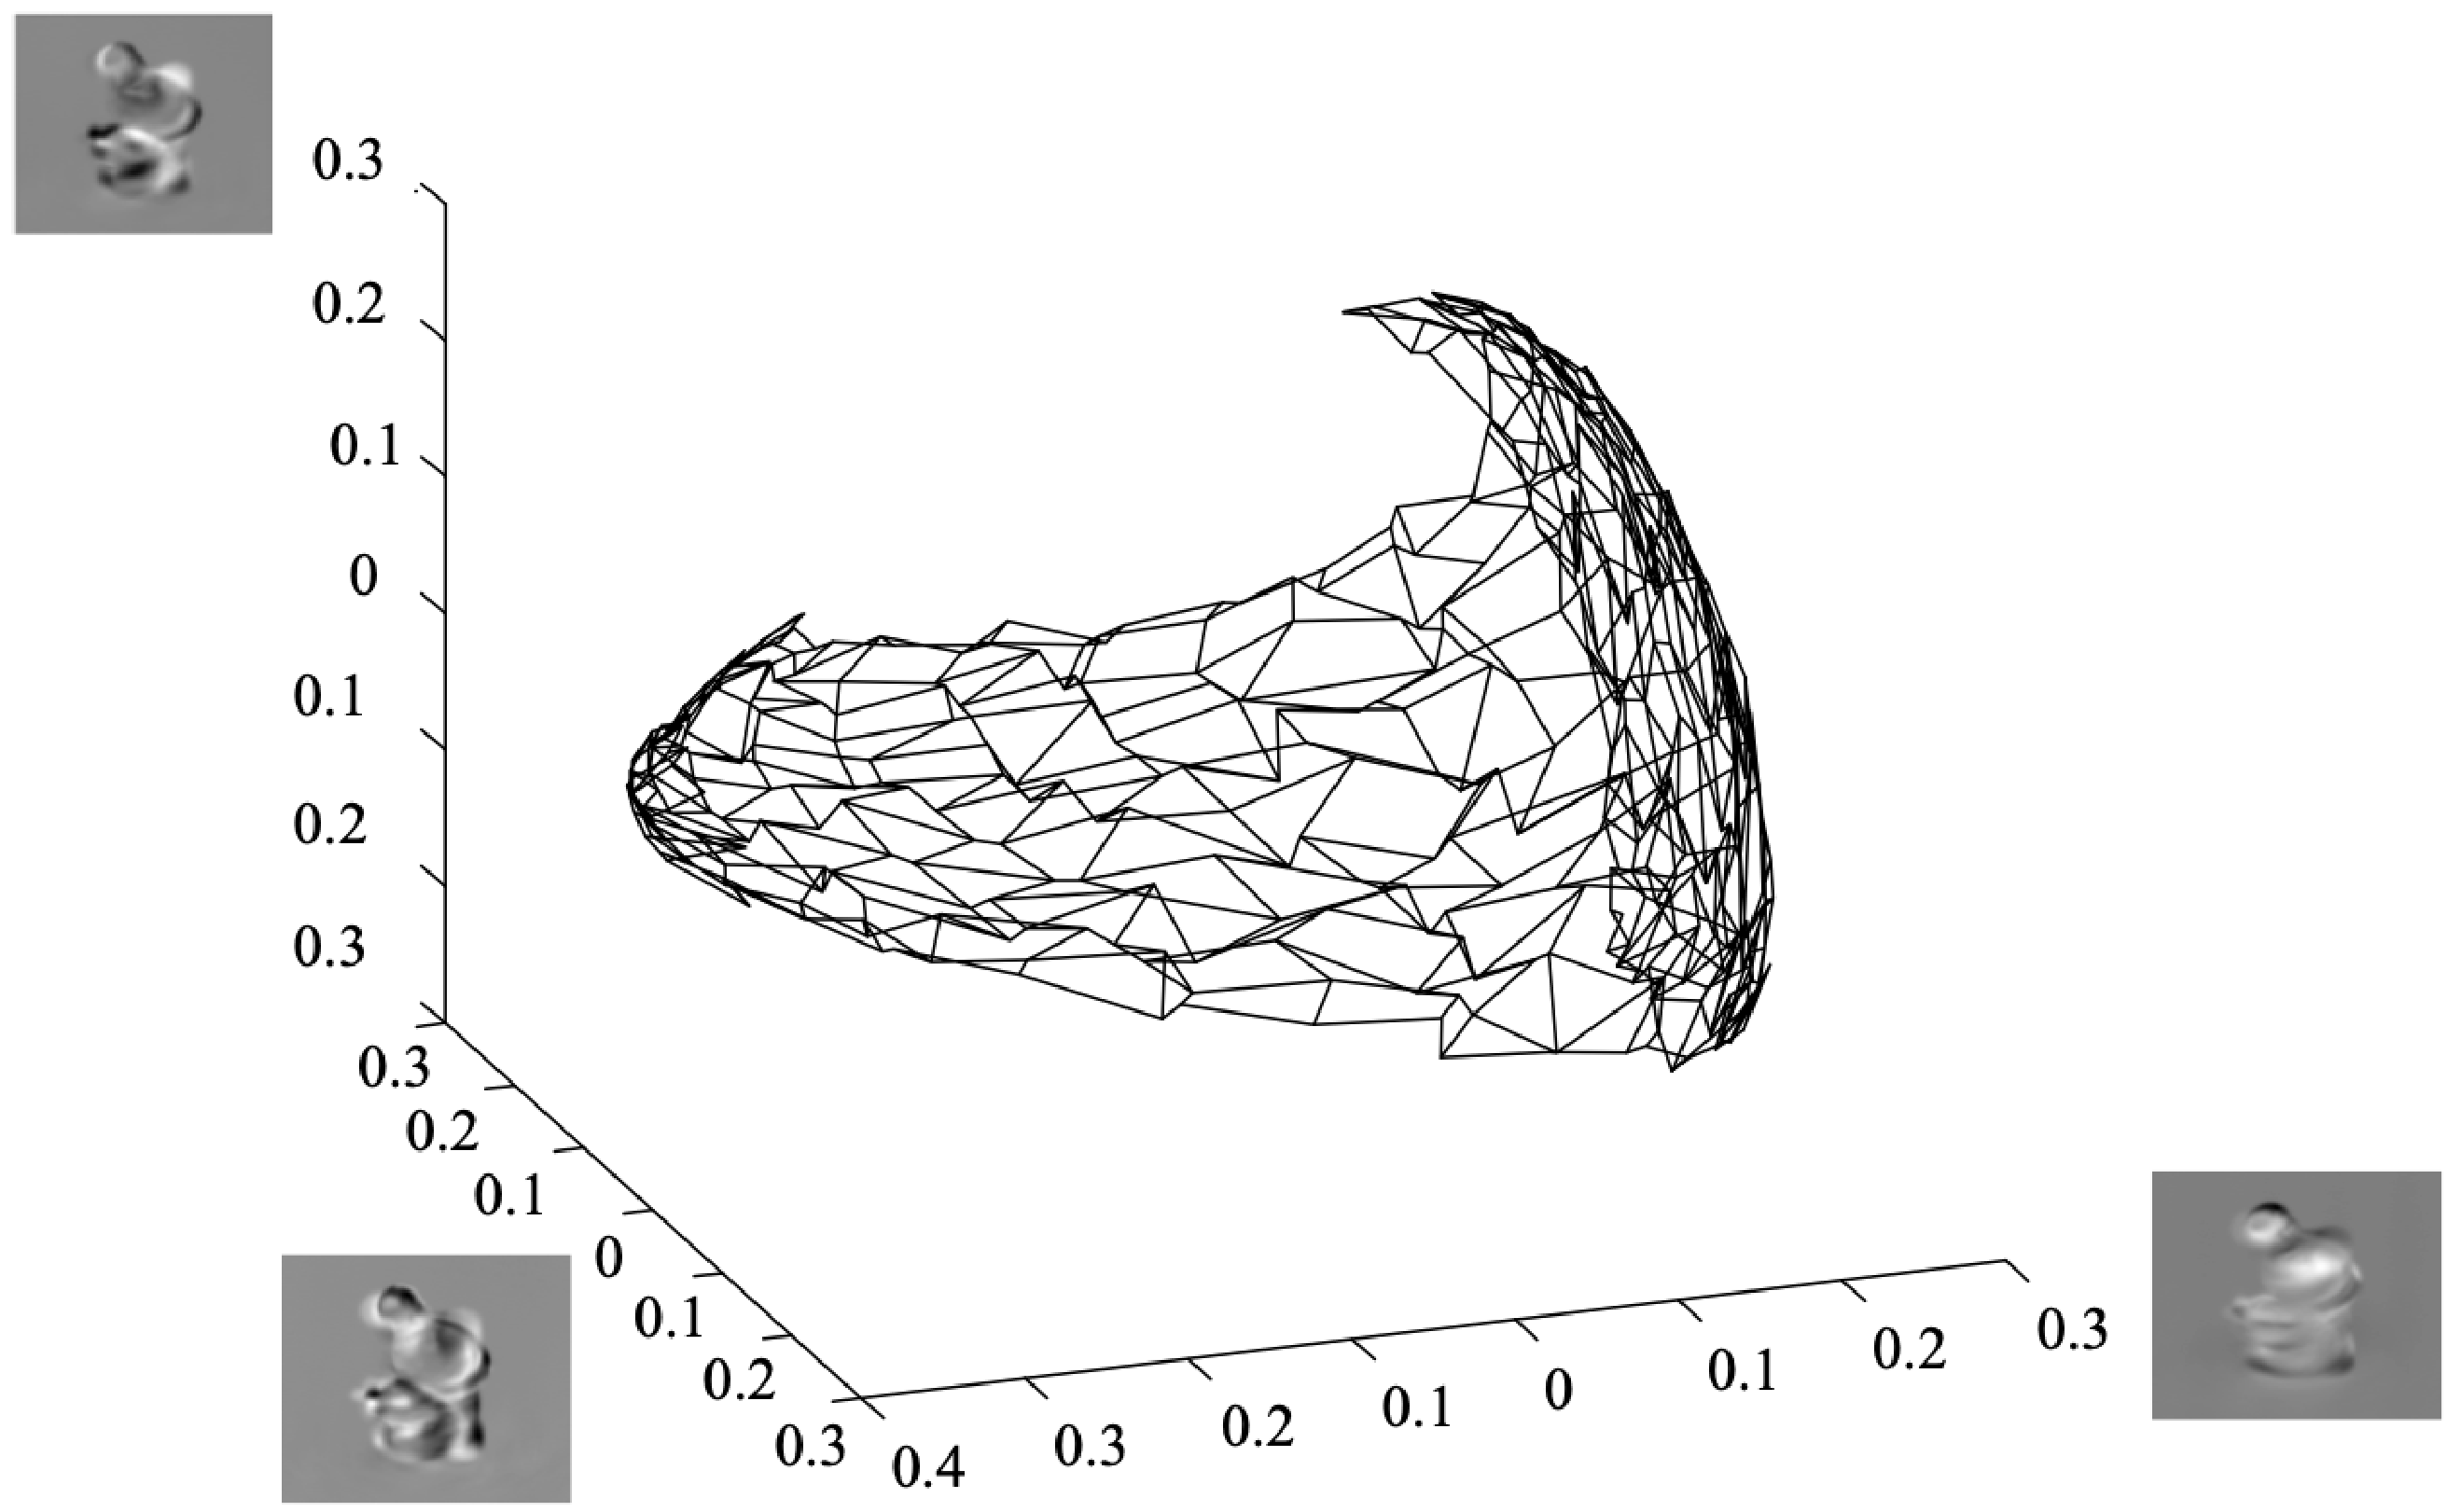
\includegraphics[height=4cm]{cca-manifold}}
\end{frame}

\section{Independent Component Analysis (ICA)}
\label{sec:ica}

\begin{frame}
  \frametitle{Independent Component Analysis (ICA)}
  \begin{itemize}
  \item ICA is a powerful technique from signal processing (blind source separation)
  \item Can we seen as an extension of PCA
  \item PCA takes statistics up to 2nd order into account
  \item ICA estimate components that are statistically independent
  \item Generates sparse/local descriptors - sparse coding
  \end{itemize}
\end{frame}

\begin{frame}
  \frametitle{Independent Component Analysis (ICA)}
  \begin{itemize}
  \item m scalar variables - $X = (x_1, ~ \ldots ~ x_m)^T$
  \item Assumed to be a linear mixture of n sources - $S = ( s_1, ~ ... ~ s_n )^T$
    \[
      X = A S
    \]
  \item Objective: Given X find estimates for A and S under the assumption S are independent
  \end{itemize}
\end{frame}

\begin{frame}
  \frametitle{ICA Example}
  \centerline{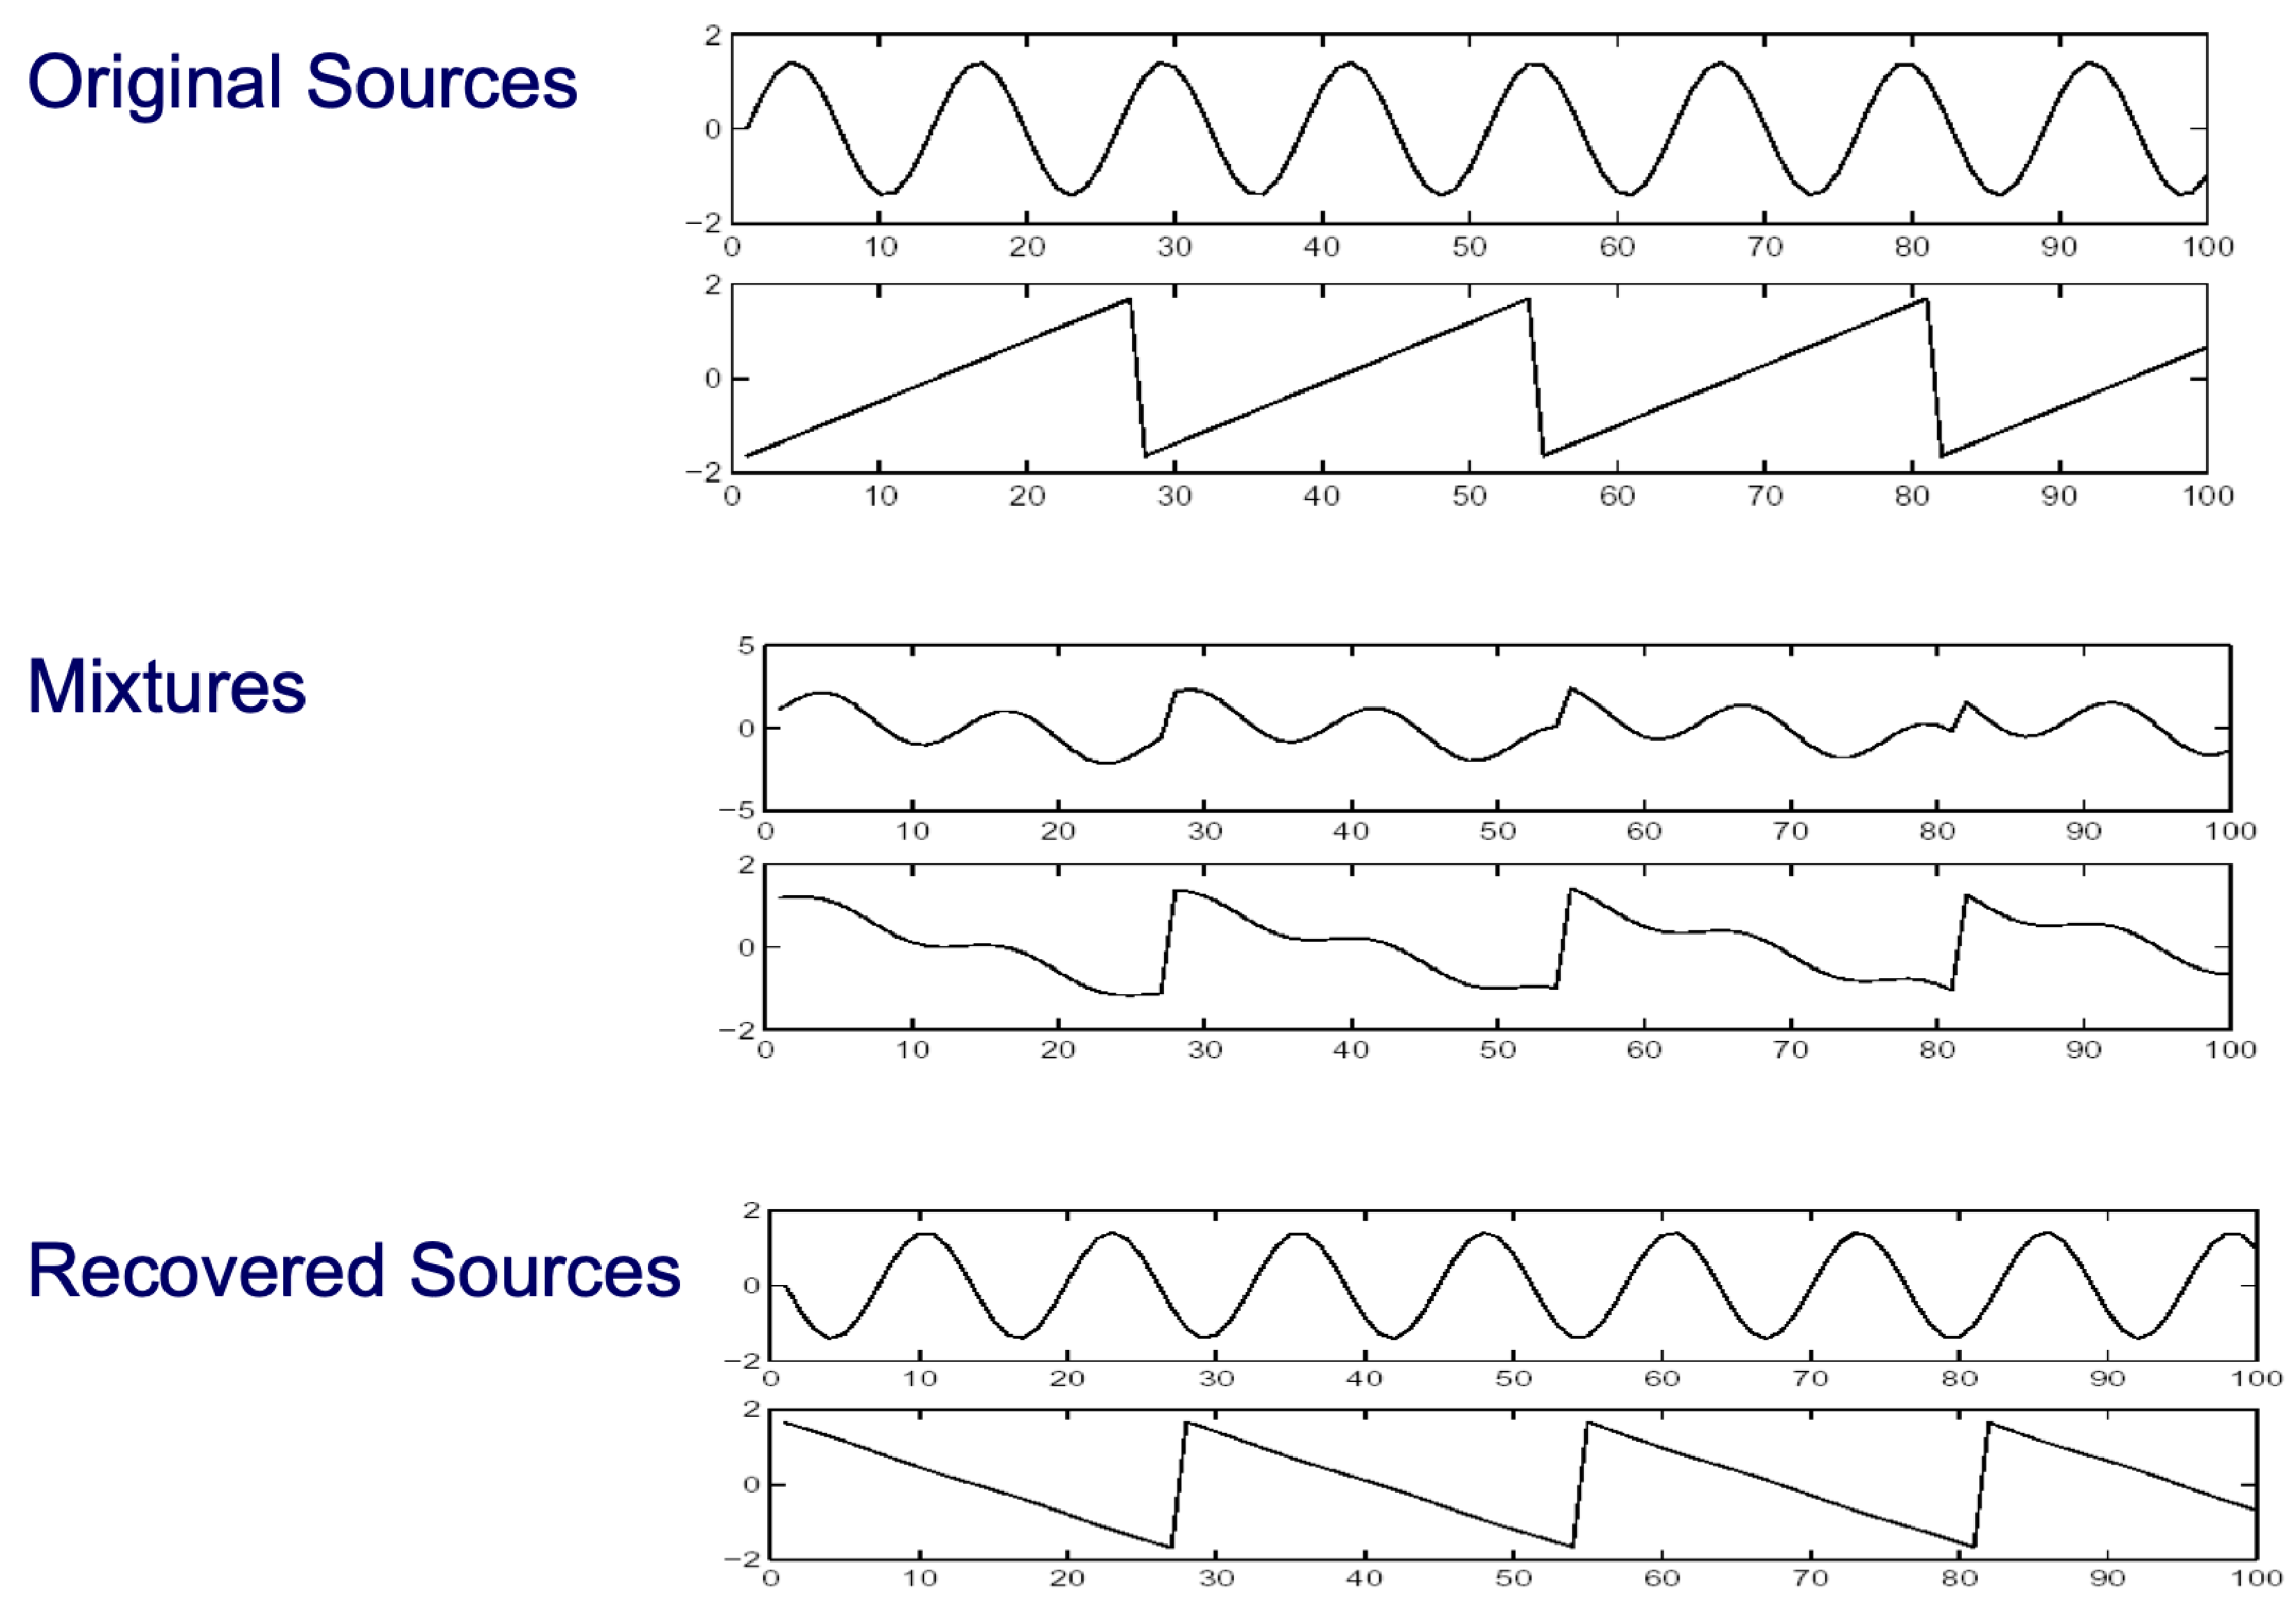
\includegraphics[height=6cm]{ica-example}}
\end{frame}

\begin{frame}
  \frametitle{ICA Example}
  \centerline{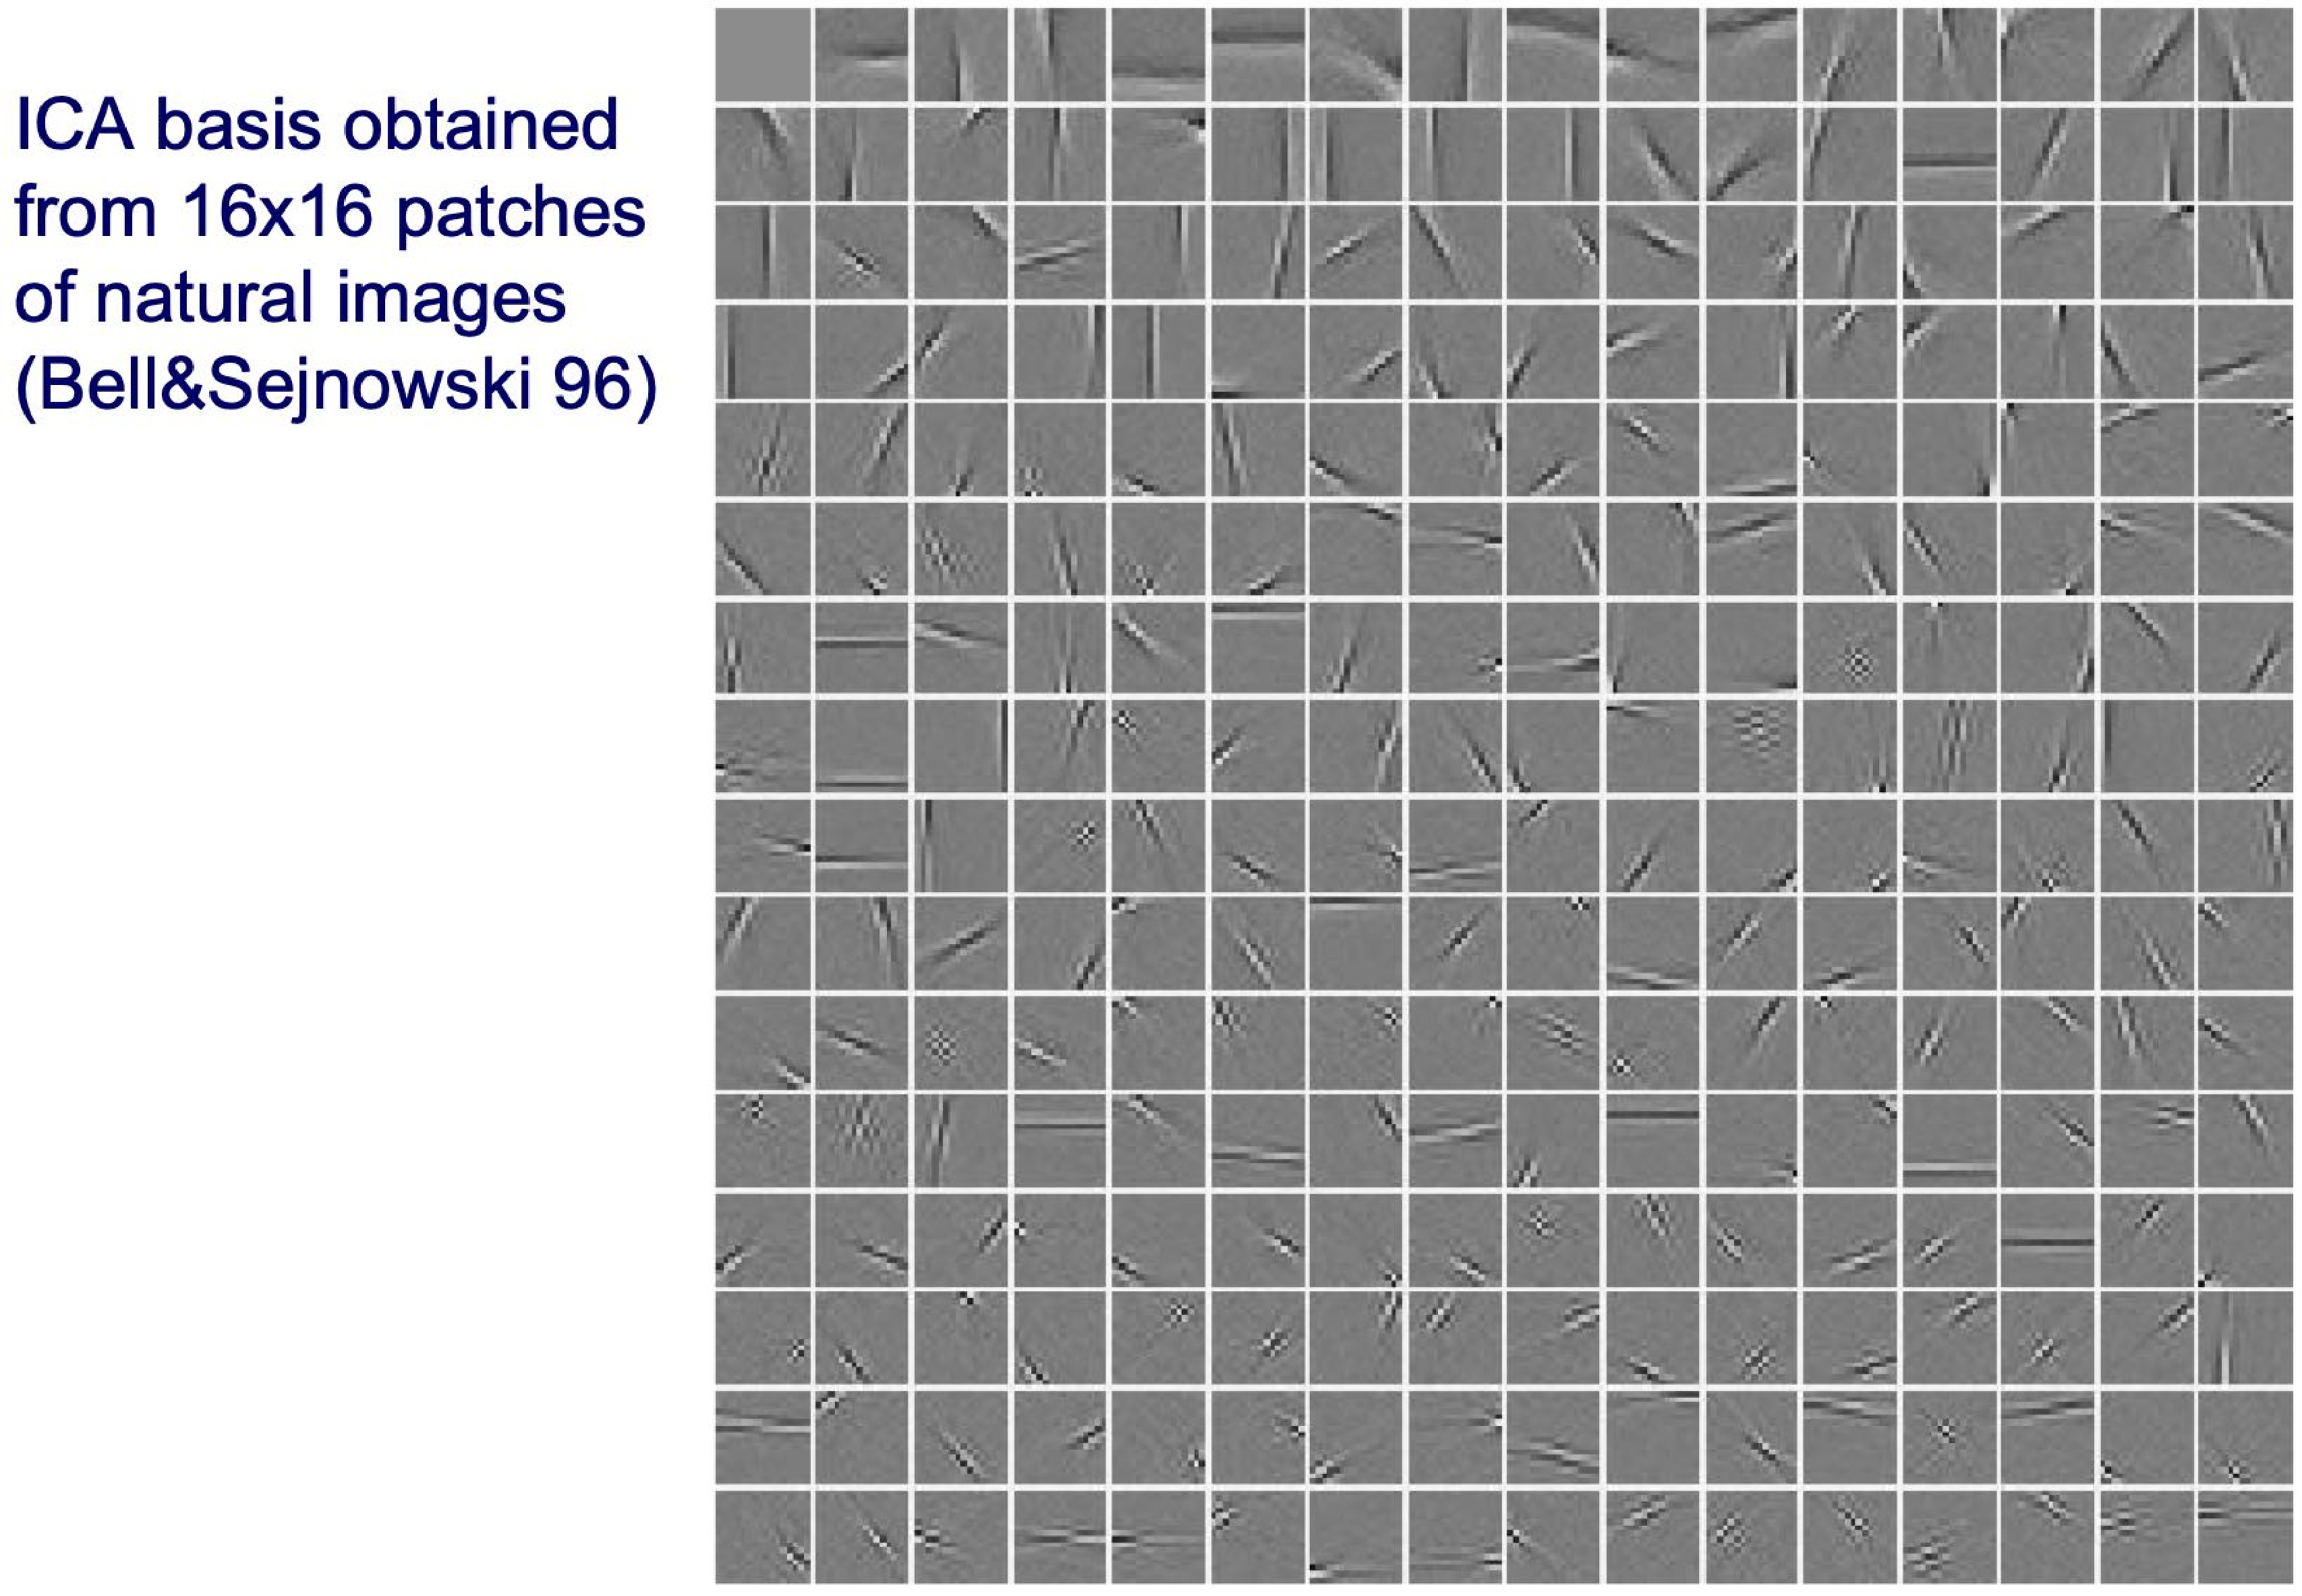
\includegraphics[height=6cm]{ica-example2}}
\end{frame}

\begin{frame}
  \frametitle{ICA Algorithms}
  \begin{itemize}
  \item Minimize a complex tensor function
  \item Adaptive algorithms based on stochastic gradient
    \begin{itemize}
    \item Measure independence
    \item Computer A recursively to maximize independence
    \end{itemize}
  \item ICA only works for non-Gaussian sources
  \item Often whitening of data is performance
  \item ICA does not provide ordering
  \item ICA components are not orthogonal
  \end{itemize}
\end{frame}

\begin{frame}
  \frametitle{ICA noise suppression example}
  \centerline{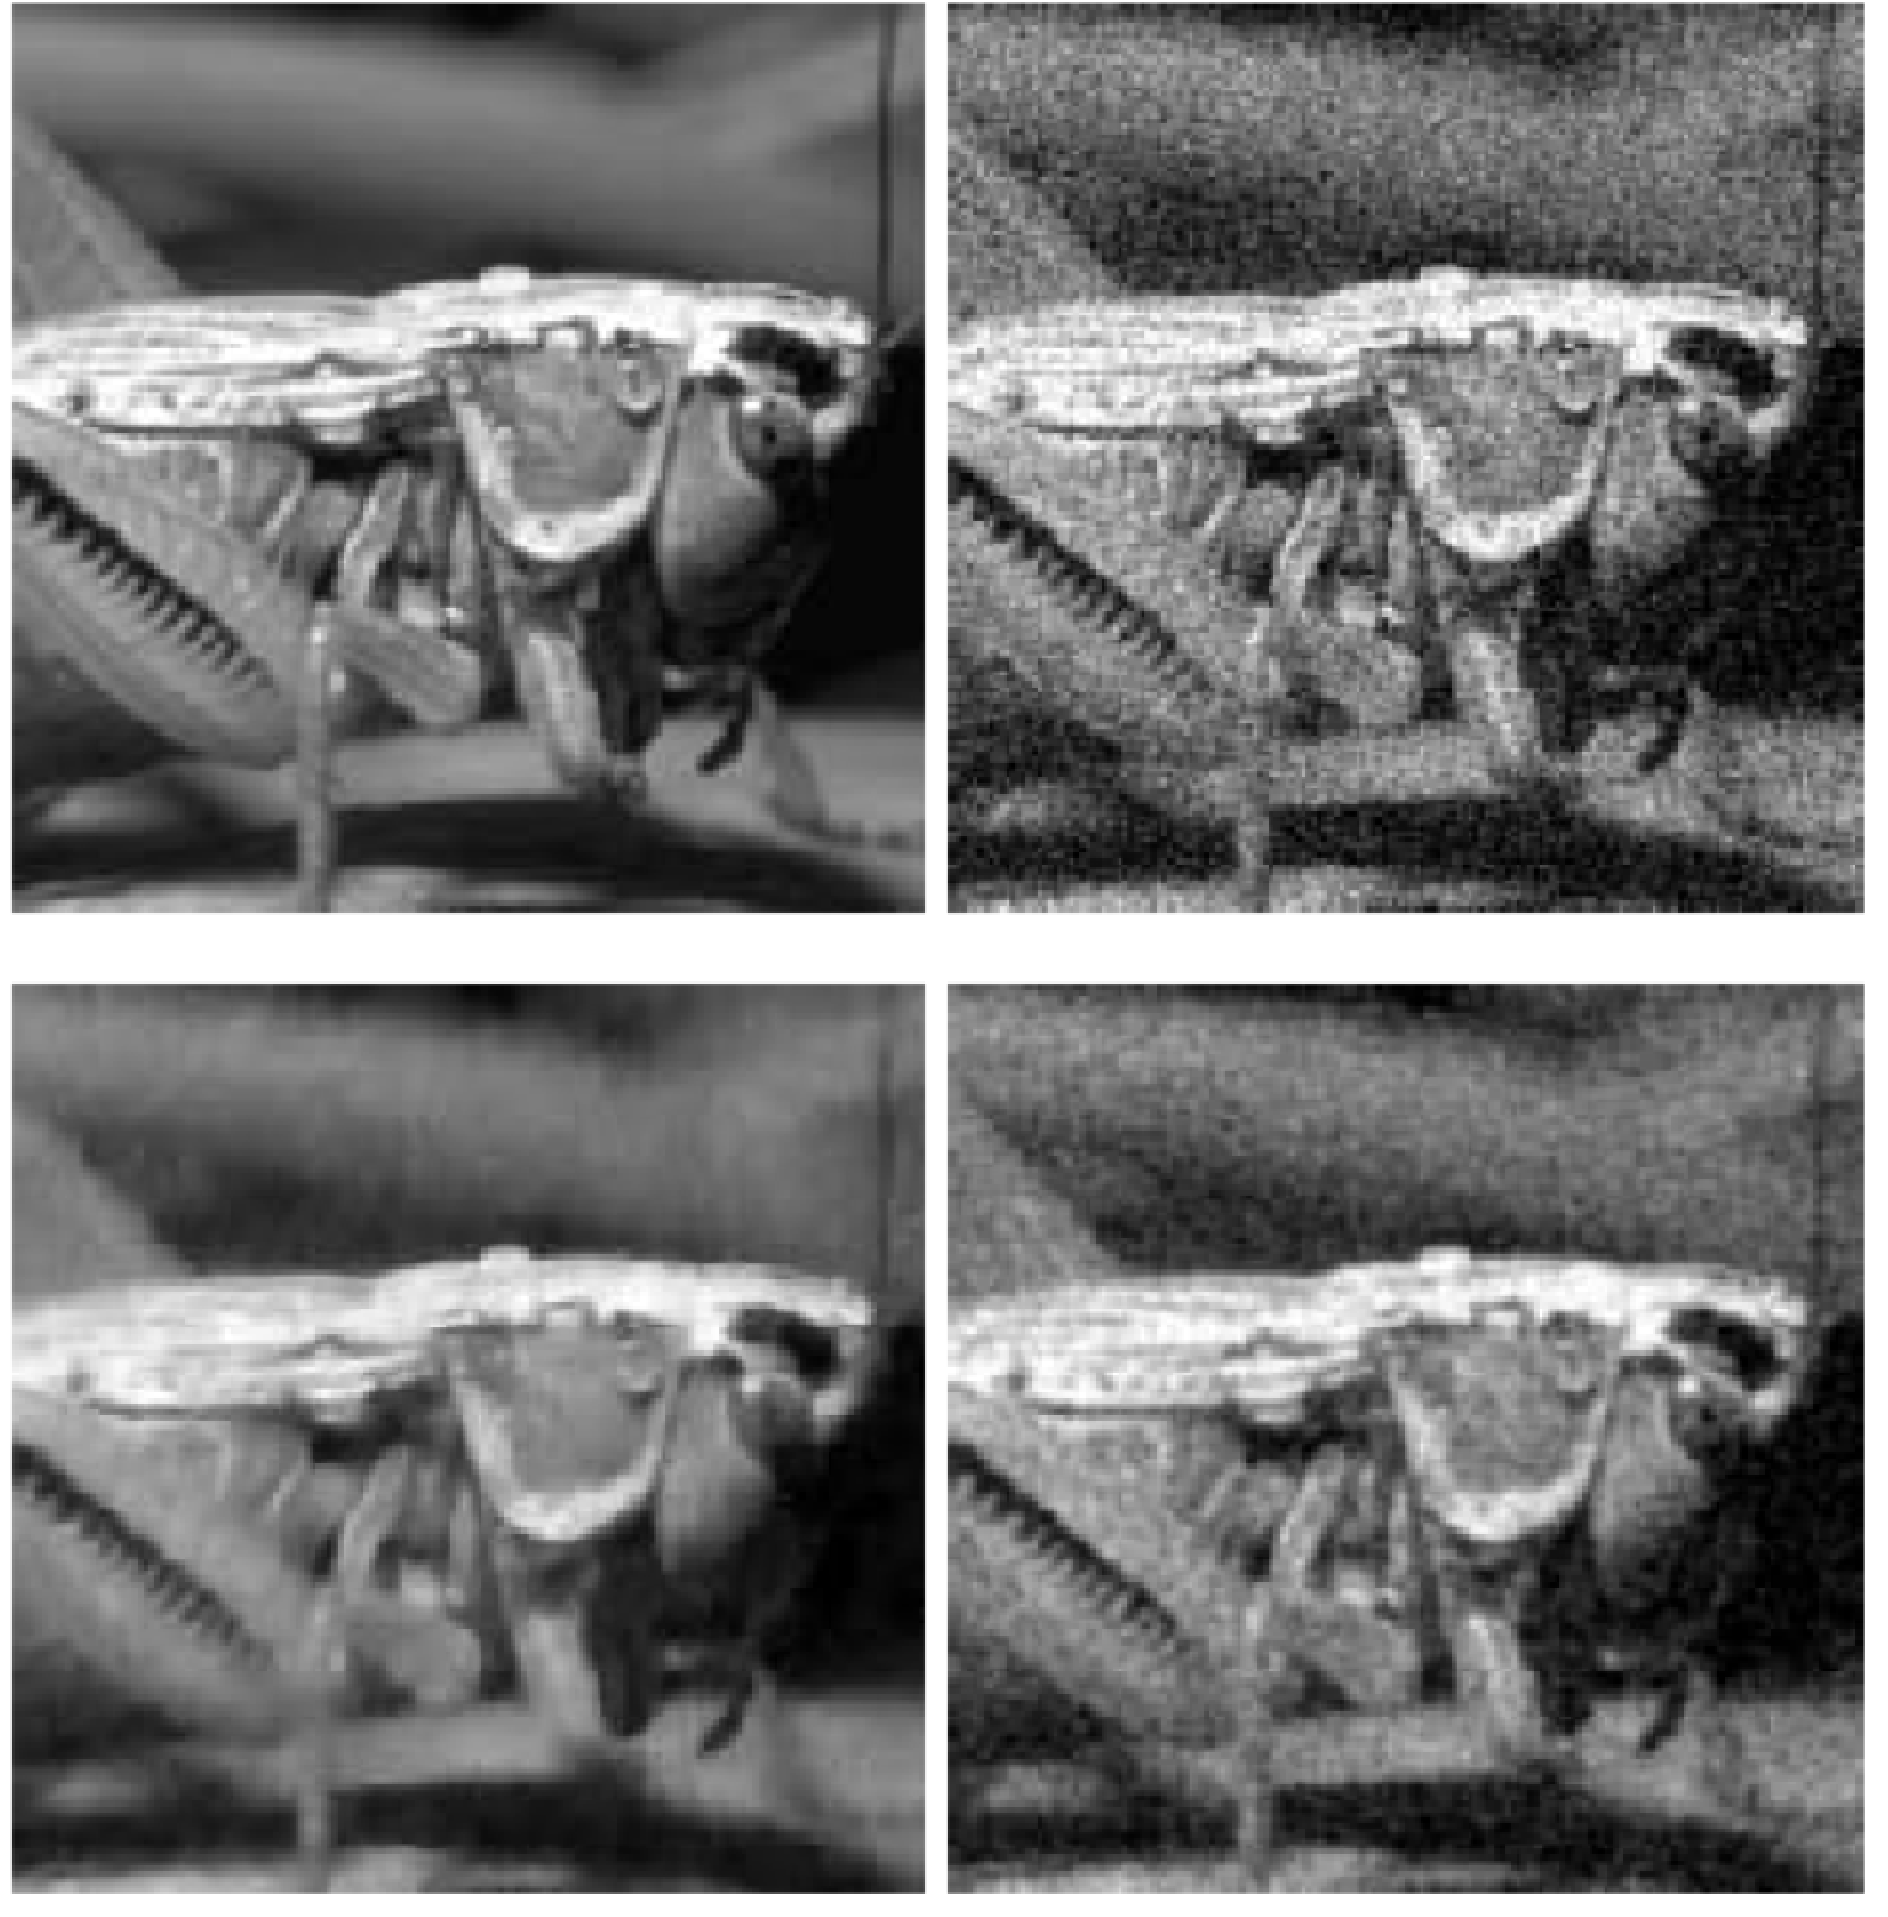
\includegraphics[height=6cm]{ica-noise-suppression}}
  \centerline{Example from Hyv{\"a}rinen, 1999}
\end{frame}

\begin{frame}
  \frametitle{PCA vs ICA for face recognition}
  \centerline{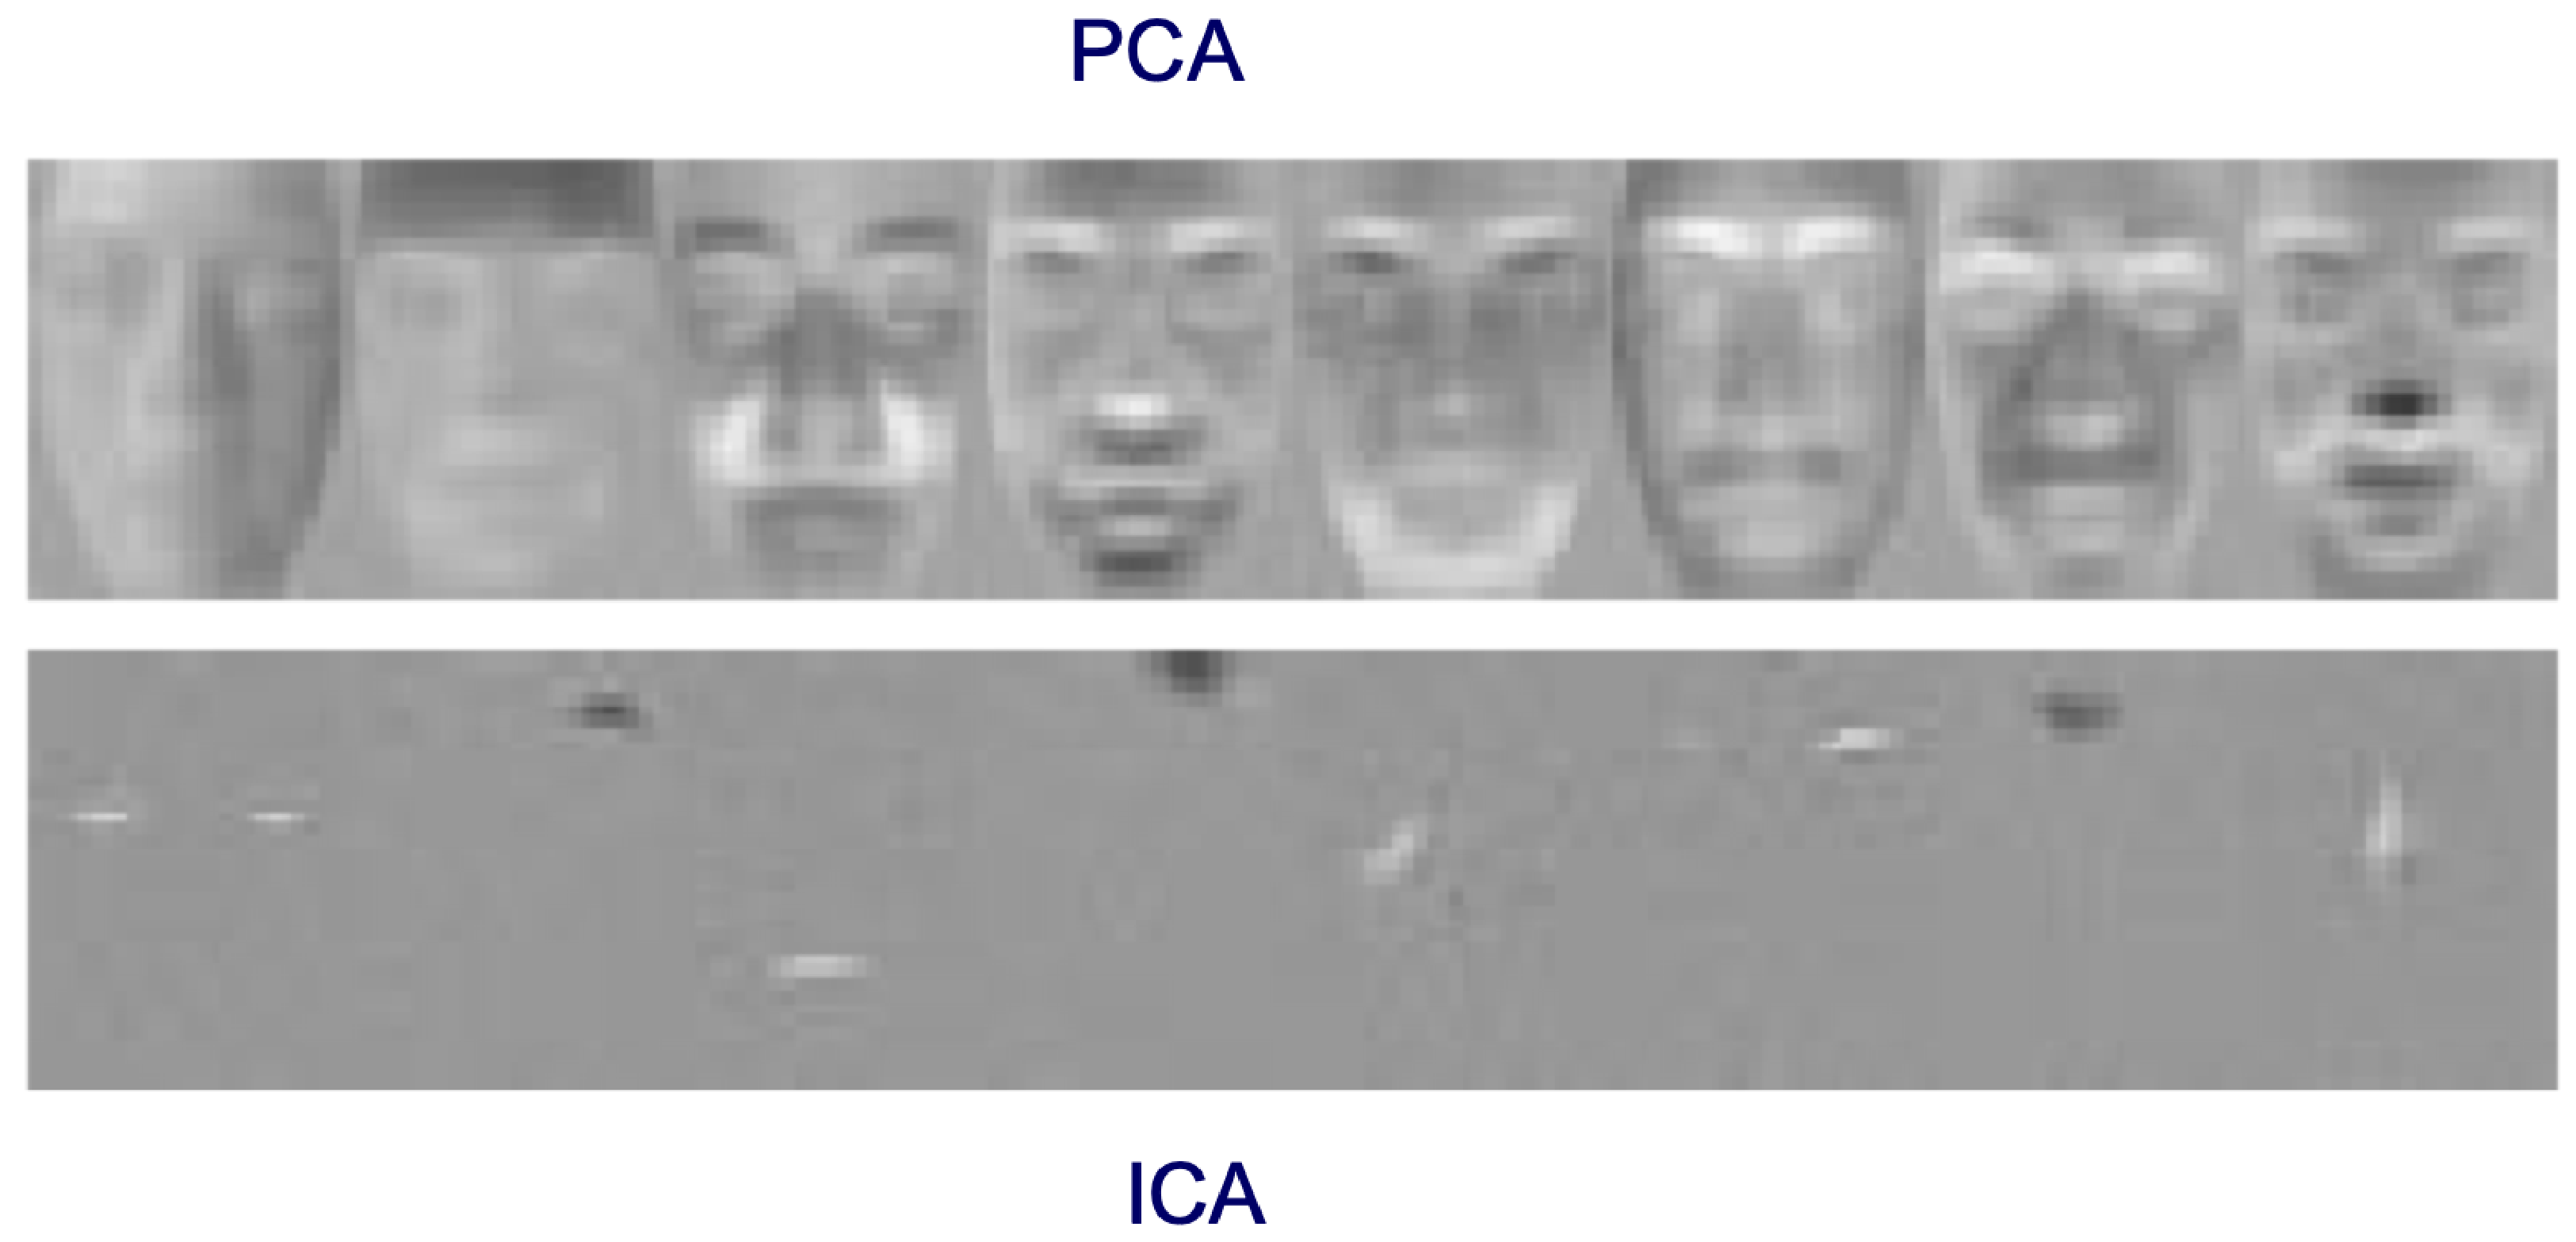
\includegraphics[height=6cm]{pca-vs-ica}}
  \centerline{From Baek et al, 2002}
\end{frame}

\section{Summary}
\label{sec:summary}

\begin{frame}
  \frametitle{Summary}
  \begin{itemize}
  \item Brief overview of use of sub-space methods for data processing
  \item The exact task should dictate the choice of methods
  \item Other cascaded processing simplifies complexity
  \item Good standard tools available in most signal processing toolboxes
  \end{itemize}
\end{frame}

\begin{frame}
  \frametitle{Questions}
  \centerline{\Huge Questions}
\end{frame}

\end{document}

%%% Local Variables:
%%% mode: latex
%%% TeX-master: t
%%% End:
